% !TeX root = KSPM_RJwrapper.tex
\title{\pkg{KSPM}: A Package For Kernel Semi-Parametric Models} % Capitalized title
\author{by Catherine Schramm, Sébastien Jacquemont, Karim Oualkacha, Aurélie Labbe and Celia M.T. Greenwood}

\maketitle

\abstract{ % 209/150 mots max
Kernel semi-parametric models and their equivalence with linear mixed models provide analysts with the flexibility of machine learning methods and a foundation for inference and tests of hypothesis. These models are not impacted by the number of predictor variables, since the kernel trick transforms them to a kernel matrix whose size only depends on the number of subjects. Hence, methods based on this model are appealing and numerous, however only a few R programs are available and none includes a complete set of features. Here, we present the \pkg{KSPM} package to fit the kernel semi-parametric model and its extensions in a unified framework. \pkg{KSPM} allows multiple kernels and unlimited interactions in the same model. It also includes predictions, statistical tests, variable selection procedure and graphical tools for diagnostics and interpretation of variable effects. Currently \pkg{KSPM} is implemented for continuous dependent variables but could be extended to binary or survival outcomes.
}

\section{Introduction}

%Introductory section which may include references in parentheses
%\citep{R}, or cite a reference such as \citet{R} in the text.

In the last decades, the popularity and accessibility of machine learning has increased as a result of both the availability of big data and technical progress in computer science. The flexibility of machine learning methods enables avoidance of assumptions about functional relationships, such as strong linear or additive hypotheses, that are often involved in classical statistical models. However, this flexibility and adaptability also limits the capacity to interpret results or make inference. When understanding and inference are required, simpler statistical models are often preferred, as they are easy to understand and implement. Methods from the machine learning field might better model complex relationships, and yet would be more attractive if the results could be made interpretable. With this goal in mind, \cite{liu2007semiparametric} clearly demonstrated the under-appreciated equivalence between a machine learning tool and a classical statistic model through the link between kernel semi-parametric models -- developed first in the machine learning field -- and more classical linear mixed models. 
This equivalence allows analysts to take advantage of knowledge advances in both the machine learning domain and the traditional statistical inference domain, including hypotheses testing, when using kernel semi-parametric models (Table~\ref{table:MLvsStat}). 


\begin{table}[htbp]
\begin{center}
\begin{tabular}{p{7cm}p{6cm}}
\toprule
\multicolumn{2}{c}{Features of kernel models} \\
\midrule
from traditional statistical models & from machine learning models \\
\midrule
\begin{itemize}
  \item Inference, confidence/prediction intervals
    \item Tests, $p$~values
    \item Information criteria (variable selection)
    \item Interpretation via estimation of functional form of variable effects on outcome
\end{itemize}
&
\begin{itemize}
    \item No need to explicitly define outcome-predictors relationship
    \item May deal with a large amount of data (big data and fat data)
    \item Potential for reinforcement learning
\end{itemize}
~\\
\bottomrule
\end{tabular}
\caption{\label{table:MLvsStat} Features of kernel models combine features from traditional statistical models and features from machine learning models.}
\end{center}
\end{table}



The kernel semi-parametric model assumes that the outcome is related to the set of variables through an unknown smooth function, which is simply approximated by computing the similarity matrix between subjects according to the set of variables and a chosen kernel function (i.e., the kernel trick). Matrix size depends only on the number of subjects, making kernel models particularly suited to datasets where the number of features is very large ($p >>n$). The equivalence between kernel semi-parametric models and linear mixed models motivates a score test, which is simple to implement, for the simultaneous effect of all variables on the outcome.




Methods based on the kernel semi-parametric model and its extensions are appealing and numerous, but only a few programs are available, and none includes a complete set of the features that correspond to recent developments. Table~\ref{table:packages} gives some examples of existing R packages according to their features of interest. 


\begin{table}[htbp]
\begin{center} 
\begin{tabular}{lclllllll}
&  \begin{turn}{80} \textbf{Adjustment} \end{turn}  &  \begin{turn}{80} \textbf{User's own kernel} \end{turn} & \begin{turn}{80} \textbf{Single kernel test} \end{turn} &  \begin{turn}{80} \textbf{Test of interaction} \end{turn}   & \begin{turn}{80} \textbf{Predictions} \end{turn}  &   \begin{turn}{80} \textbf{Interpretation plot} \end{turn} & \begin{turn}{80} \textbf{Diagnostic plots} \end{turn} &   \begin{turn}{80} \textbf{Variable selection} \end{turn}  \\ 
\toprule
\pkg{coxme} & \checkmark & \checkmark &            &            &            &            &            &            \\
\pkg{SKAT} &            &    \checkmark   & \checkmark &            &            &            &            &            \\
SPA3G &            &            &            & \checkmark &            &            &            &            \\
\pkg{KRLS} &            &            &            &            & \checkmark & \checkmark  &            &            \\
\pkg{e1071} &  &  & &  & \checkmark & \\
\midrule
\pkg{KSPM}  & \checkmark & \checkmark & \checkmark &\checkmark & \checkmark & \checkmark & \checkmark & \checkmark \\
\bottomrule
\end{tabular}
\caption{\label{table:packages} Features incorporated in \CRANpkg{KSPM}~\citep{schrammPackage}, as well as in several other R packages for kernel nonparametric or semiparametric models: \CRANpkg{coxme}~\citep{coxmeTherneau}, \CRANpkg{SKAT}~\citep{SKATLee}, \CRANpkg{KRLS}~\citep{KRLSpackageR}, \CRANpkg{e1071}~\citep{e1071} and \CRANpkg{SPA3G}~\citep{SPA3GLi}. \textbf{Adjustment} refers to models including a kernel for adjusting the model on correlation structure similarly to a random factor. \textbf{User's own kernel} refers to a kernel function explicitly defined by the user of the package, in contrast to traditional kernel functions that are already implemented in the package. \textbf{Single kernel test} refers to the test of the joint effect of a set of variables on the outcome. \textbf{Test of interaction} refers to the interaction between two sets of variables and its effect on the outcome. \textbf{Predictions} refers to the possibility of displaying predictions with confidence and prediction intervals. \textbf{Interpretation plot} refers to graphical tools for interpretation of individual effects of each variable in the kernel on the outcome. \textbf{Diagnostic plots} refers to graphical tools based on residuals and leverage measures to check the validity conditions of a model and identify outlier samples. \textbf{Variable selection} refers to the implementation of a variable selection procedure.} 
\end{center}
\end{table}


Several packages in Table \ref{table:packages} were developed in the genetics field where interest often lies in testing the contribution of a group of variables (variants) simultaneously, notably through the sequence kernel association test (SKAT) for single nucleotide polymorphisms~\citep{wu2011rare, chen2016small}. Extensions from single to multiple kernel model were motivated by (i) interaction tests~\citep{li2012gene, wang2017set, ge2015kernel, marceau2015fast} and (ii) estimating the conditional effect of one set of variables after adjusting for another set of variables, or after adjusting for population structure~\citep{oualkacha2013adjusted}. The latter goal may be achieved easily using the \code{lmekin()} function from the \pkg{coxme} package under mixed model theory where kinship matrix corresponds to the kernel matrix measuring similarity between subjects, and defines the covariance matrix of the random effect term. 


In the machine learning field, packages like \pkg{e1071} have been developed to perform accurate predictions and they focus on a single kernel function. Traditionally, model interpretation has remained an outstanding challenge of the machine learning field. However it has been recently demonstrated that the kernel semi-parametric models can be used to interpret effects of variables on the outcome through a graphical tool based on derivatives~\citep{hainmueller2013kernel} and this is implemented in the \pkg{KRLS} package. When the kernel function and the corresponding approximated smooth function are differentiable with respect to the variable of interest, pointwise derivatives capture the effect of this variable on the outcome. 

Since researchers may be interested in all of these features, we have consolidated them in the R package \pkg{KSPM}. The package and a vignette including detailed examples are available from the comprehensive R archive network (CRAN) at https://CRAN.R-project.org/package=KSPM. Our package, currently designed for continuous outcomes and normal errors, fits kernel semi-parametric models and their extensions in a unified framework incorporating all the previously described model fitting features and tests. It allows multiple kernels and unlimited interactions in the same model. Although most popular kernel functions are available in the package, the user also has the option of designing and using his/her own kernel functions. Furthermore, whenever interest lies in prediction or making inference from the model, diagnostic assessments of the model may be performed through graphical tools to detect data points with large residuals or high leverage that may greatly influence the results. Finally, we have also included a variable selection procedure based on Akaike's and Bayesian information criteria (AIC and BIC). These last two options are not included in other software packages.


The \pkg{KSPM} package is a new tool for semi-parametric regression. It is not competing with other R packages for semi- or non-parametric regression models since either our methods or our objectives are different. Indeed, the estimation method involved in \pkg{KSPM} is based on regularized least squares in the kernel Hilbert space and should not be confused with local kernel smoothing based on Nadaraya-Watson estimator (\CRANpkg{np} package, \cite{npPackage}). Similarly, \pkg{KSPM} is also different from other smoothing methods connecting regression segments through knots among which we may cite splines (\CRANpkg{mgcv} package, \cite{mgcvPackage}). 

However, since the kernel semi-parametric model is equivalent to a linear mixed effect model, our package could be compared to \CRANpkg{lme4}~\citep{lme4package} or \CRANpkg{nlme}~\citep{nlmePackage} packages for linear mixed effect models. Although it is possible to obtain similar inference from any variables involved in a linear part of each model, and to obtain similar predictions from both overall models, loss function maximization are different. Moreover, \pkg{KSPM} has the advantage of being easier-to-use as the user does not need to compute kernel matrix nor matrix of interactions and provides interpretations for variable effects that cannot be obtained with traditional packages.




\section{Kernel semi-parametric models}

\subsection{Single kernel semi-parametric model} \label{sec:models-notations-skspm}

Let $Y = (Y_1, ..., Y_n)^\top$ be a $n \times 1$ vector of continuous outcomes where $Y_i$ is the value for subject $i$ ($i = 1, ..., n)$, and $X$ and $Z$ are $n \times p$ and $n \times q$ matrices of predictors, such that $Y$ depends on $X$ and $Z = (\mathbf{z_{.1}} , ..., \mathbf{z_{.q}})$ as follows:
\begin{equation} \label{eq:kspm}
Y = X\beta + h(Z) + e
\end{equation}
where $\beta$ is a $p \times 1$ vector of regression coefficients for the linear parametric part, $h(.)$ is an unknown smooth function and $e$ is an $n \times 1$ vector of independent and homoscedastic errors such as $e_i \sim \mathcal{N}(0, \sigma^2)$. Throughout this article, $X\beta$ will be referred to as the linear part of the model and we assume that $X$ contains an intercept. $h(Z)$ will be referred to as the kernel part. The function $h(.)$ need not be explicitly specified but it is assumed to lie in $\mathcal{H}_k$, the function space generated by a kernel function $k(.,.)$ which is, by definition, symmetric and positive definite. We note that $K$, the $n \times n$ Gram matrix of $k(.,.)$ such that $K_{ij} = k(\mathbf{z_{i.}}, \mathbf{z_{j.}})$, represents the similarity between subjects $i$ and $j$ according to $Z$. Of note, in the estimation process, $h(.)$ will be expressed as a linear combination of $k(.,.)$ (see Equation~(\ref{eq:representer})). See "Fitting the kernel semi-parametric model with \code{kspm}" for straightforward coding.

\subsection{The multiple kernel semi-parametric model} \label{sec:models-notations-mkspm}

Now suppose there are $L$ matrices $Z_1, ..., Z_L$ of dimension $n \times q_1$, ..., $n \times q_L$ respectively. Keeping a similar notation, $Y$ can be assumed to depend on $X$ and $Z_1$, ..., $Z_L$ as follows:
\begin{equation} \label{eq:mkspm}
Y = X\beta + \sum\limits_{\ell = 1}^L h_{\ell}(Z_{\ell}) + e
\end{equation}
where $\forall \ell \in \left\lbrace 1, ..., L \right\rbrace$, $h_{\ell}$ is an unknown smooth function from $\mathcal{H}_{k_{\ell}}$, the function space generated by a kernel function $k_{\ell}(.,.)$ whose Gram matrix is noted $K_{\ell}$. We assume $\forall \ell \neq m$, $h_{\ell}(Z_{\ell}) \neq h_{m}(Z_{m})$ either because $Z_{\ell} \neq Z_{m}$ or $k_{\ell}(.,.) \neq k_{m}(.,.)$ or both. Note that when $L = 1$, the model corresponds to Equation~(\ref{eq:kspm}).


Suppose there is an interaction between two sets of variables represented by $Z_1$ and $Z_2$,  $n \times q_1$ and $n \times q_2$ matrices, and $Y$ depends on $X$, $Z_1$ and $Z_2$ as follows:
\begin{equation} \label{eq:ikspm}
Y = X\beta + h_1(Z_1) + h_2(Z_2) + h_{12}(Z_1, Z_2) + e
\end{equation}
where $h_1(.)$, $h_2(.)$ and $h_{12}(.,.)$ are unknown smooth functions from $\mathcal{H}_{k_1}$, $\mathcal{H}_{k_2}$ and $\mathcal{H}_{k_{12}}$ respectively. The $h_{12}(.,.)$ function represents the interaction term if its associated kernel function $k_{12}(.,.)$ is defined as the product of kernel functions $k_1(.,.)$ and $k_2(.,.)$ as follows:
\begin{equation}
\label{eq:inter}
k_{12}\left((Z_1, Z_2)_i, (Z_1, Z_2)_j\right) = k_1(\mathbf{z_{1i.}}, \mathbf{z_{1j.}}) \times k_2(\mathbf{z_{2i.}}, \mathbf{z_{2j.}})
\end{equation}
such that $K_{12} = K_1 \odot K_2 $ where $\odot$ is the Hadamard product~\citep{ge2015kernel}. Model~(\ref{eq:ikspm}) is a particular case of the multiple kernel semi-parametric model~(\ref{eq:mkspm}) with $L=3$, $Z_3 = (Z_1, Z_2)$, $q_3 = q_1 + q_2$ and $h_{3}$ = $h_{12}$. Of notes, in \pkg{KSPM}, different kernel choices can be made for $k_1(.,.)$ and $k_2(.,.)$. Obviously, this 2-way interaction model could be generalized to higher order interaction terms in a similar manner.





\subsection{Link with linear mixed models} \label{sec:models-notations-lme}

As shown by \cite{liu2007semiparametric}, model~(\ref{eq:mkspm}) is equivalent, without additional conditions, to the following linear mixed model:
\begin{equation} \label{eq:lmm}
Y = X\beta + \sum\limits_{\ell = 1}^L h_{\ell} + e
\end{equation}
where $\forall \ell \in \left\lbrace 1,...,L\right\rbrace$, $h_{\ell} \sim \mathcal{N}(0, \tau_{\ell} K_{\ell})$ with %$\tau_{\ell} = \lambda_{\ell}^{-1}\sigma^2$ and 
$K_{\ell}$ is a matrix of similarity between subjects as defined in model~(\ref{eq:mkspm}). Throughout the paper, we denote the variance parameters as $\theta = (\tau_{1}, ..., \tau_L, \sigma^2)$  and $\Sigma_{\theta} = \sum\limits_{\ell = 1}^L \tau_{\ell}K_{\ell} + \sigma^2 I$, the variance-covariance matrix of $Y$, where $I$ is the $n \times n$ identity matrix.


\subsection{Estimation of parameters}  \label{sec:models-estimation}

The parameter estimates can be obtained either by maximizing the penalized log-likelihood associated with the kernel semi-parametric model~(\ref{eq:mkspm}), or the log-likelihood derived from the corresponding linear mixed model~(\ref{eq:lmm}) \citep{liu2007semiparametric}. Even though the latter option may be computationally less time-consuming, we implemented the \pkg{KSPM} package using a penalized log-likelihood associated with the kernel semi-parametric model, because this method leads to an estimation of $h$ useful for prediction, and also leads to suitable approaches for interpretation through kernel derivatives. Estimation of parameters is obtained by maximizing the penalized log-likelihood function:
\begin{equation} \label{eq:pll}
l(\beta, h) = -\frac{1}{2}\sum\limits_{i = 1}^n \left(Y_i - X_i^\top\beta - \sum\limits_{\ell = 1}^L h_{\ell}(Z_{\ell i}) \right)^2 - \frac{1}{2}\sum\limits_{\ell = 1}^L \lambda_{\ell} \parallel h_{\ell}\parallel_{\mathcal{H}_{k_{\ell}}}^2
\end{equation}
where $\lambda_1$, ..., $\lambda_L$ are tuning parameters associated with each smooth function $h_1(.)$, ..., $h_L(.)$ and $\parallel .\parallel^2_{\mathcal{H}_{k_{\ell}}}$ defines the inner product on $\mathcal{H}_{k_{\ell}}$ space. According to the Representer theorem \citep{kimeldorf1971some}, the functions $h_1$, ..., $h_L$ satisfying Equation~(\ref{eq:pll}) can be expressed as:
\begin{equation}\label{eq:representer}
\forall \ell \in \left\lbrace 1,...,L \right\rbrace, \quad h_{\ell}(.) = \sum\limits_{i=1}^n \alpha_{\ell i} k(., Z_{\ell i})
\end{equation}
where $\forall \ell \in \left\lbrace 1,...,L \right\rbrace$, $\alpha_{\ell} = (\alpha_{\ell 1}, ..., \alpha_{\ell n})^\top$ is a $n \times 1$ vector of unknown parameters.
Estimating the kernel semi-parametric model parameters consists in estimating $\alpha_1, ..., \alpha_L$ and $\beta$. Then, estimators of $h_1(.)$, ..., $h_L(.)$ are deduced from $\hat{\alpha}_1, ..., \hat{\alpha}_L$. 



In \pkg{KSPM}, we estimate penalization parameters by minimizing the mean sum of squares of the leave-one-out errors (LOOE). An advantage of LOOE compared to other cross-validation methods is that we do not need to recompute new model(s), because its value may be derived directly from the primary model parameters:
\begin{equation} \label{eq:looe}
\forall i \in \left\lbrace 1, ..., n\right\rbrace, \qquad \text{LOOE}_i(\lambda_1, ...,\lambda_L) =  \frac{Y_i - \hat{Y}_i}{1-H_{ii}}
\end{equation}
where $H_{ii}$ is the $i^{th}$ diagonal element of the Hat matrix $H$ such as $\hat{Y} = H Y$. 


Penalization parameters and tuning parameters, if applicable, are estimated simultaneously during the optimization algorithm, by minimizing the LOOE. If only one parameter needs to be estimated, the convexity of the function to be minimized makes the problem easier and the convergence faster. In that case, \pkg{KSPM} uses the standard \code{optimize()} function from the basic R package, based on the golden section search algorithm \citep{brent2013algorithms}. When several hyperparameters need to be estimated, the resulting function to be minimized may not be convex. Hence, more complex optimization algorithms should be envisaged, and \pkg{KSPM} uses the \code{DEoptim()} function from the \CRANpkg{DEoptim} package~\citep{DEoptimPackage} based on the differential evolution algorithm \citep{mullen2009deoptim}. Given the random nature of the algorithm, it would be safe to apply the algorithm several times to ensure convergence toward the global minimum.



\subsection{Tests of hypotheses in \pkg{KSPM}}  \label{sec:models-tests}

For either a single kernel or a multiple kernel semi-parametric model, a standard test of interest is $H_0: h_{\ell}(.) = 0$, i.e., there is no effect, singly or jointly, of a set of variables on the outcome. Following \cite{liu2007semiparametric}, this test is equivalent to $H_0: \tau_{\ell} = 0$, a test of the variance component in the linear mixed model~(\ref{eq:lmm}) using the REML-based score test. The corresponding test statistic $Q_{\ell}$ follows a mixture of independent chi-square distributions with one degree of freedom \citep{zhang2003hypothesis}. 
The \pkg{KSPM} package uses exact distribution of $Q_{\ell}$ in single kernel model but in multiple kernel model, we use Davies' method to approximate this distribution \citep{davies1980distribution}. Based on similar methodology, \pkg{KSPM} also provides the global test for multiple kernel semi-parametric models $H_0: h_1(.) = ... = h_L(.) = 0$ i.e., $H_0: \tau_1 = ... = \tau_L = 0$.

\subsection{Interpretation of variable effects}  \label{sec:models-interpret}

A kernel represents similarity between subjects through combining a set of variables in a possibly complex way, that may include their possible interactions. Hence the general effect of a kernel on an outcome is hard to see and difficult to interpret. Nevertheless, the marginal effect of each variable in the kernel may be illustrated using a partial derivative function \citep{hainmueller2013kernel}. Indeed, the derivative measures how the change in a variable of interest impacts the outcome in an intuitively understandable way. When a variable's effect is linear, the interpretation is straightforward since the derivative corresponds to standard slope ($\beta$) coefficients. In kernel semi-parametric models, we are simultaneously modeling a set of variables. Therefore, when exploring the effect of any one  variable of interest, the other variables in the kernel must be taken into account. Thus, plotting pointwise derivatives of the prediction for each subject against the value of the variable of interest may help in interpreting the effect of this variable on the outcome. Although a variable-level summary statistic may be obtained by averaging the pointwise derivatives across subjects \citep{hainmueller2013kernel}, we did not implement this option in \pkg{KSPM} because the average can mask relevant variability. For example, when positive and negative derivatives occur for the same variable, the average may be zero.


\subsection{The choice of kernel functions}  \label{sec:models-functions}

In any kernel semi-parametric model, the smooth unknown function $h_{\ell}(.)$ is approximated using basis functions from $\mathcal{H}_{k_{\ell}}$. Since the inner product of the basis functions corresponds to the kernel function $k_{\ell}(.,.)$, the choice of the kernel determines the function space used to approximate $h_{\ell}(.)$. The \pkg{KSPM} package includes the most popular kernel functions, described below. The linear kernel function $ k(Z_i, Z_j) = Z_i^\top Z_j$ assumes that variables have a linear effect on outcome. It generates a linear function space so that the kernel semi-parametric model leads to a penalized multiple linear model using an $L^2$ norm (equivalent to a ridge regression). The polynomial kernel function $ k(Z_i, Z_j) = (\rho \, Z_i^\top Z_j + \gamma)^d$ assumes that $d^{th}$-order products of the variables have a linear effect on the outcome, and is equivalent to a $d^{th}$-order interaction model. The Gaussian kernel function $k(Z_i, Z_j) = exp(-\parallel Z_i - Z_j\parallel^2 / \rho)$ generates the infinite function space of radial basis functions. The sigmoid kernel function $k(Z_i, Z_j) = tanh(\rho \, Z_i^\top Z_j + \gamma)$ and the inverse quadratic kernel $k(Z_i, Z_j) = (\parallel Z_i - Z_j\parallel^2 + \gamma)^{-1/2}$ are also often cited in the literature. Finally, we propose also the equality kernel $k(Z_i, Z_j) = 1 \; \text{if} \; Z_i = Z_j \; \text{and}  \; 0 \; \text{otherwise}$. Of note, users can define their own kernel function in \pkg{KSPM} by providing the corresponding kernel matrix. Some kernel functions, such as the linear or polynomial kernels, make assumptions about the shape of the effect of the variables on the continuous outcome, whereas other kernels like the gaussian may, in theory, handle all types of effects, regardless of their complexity. Indeed, in contrast to the linear and polynomial kernels, the gaussian kernel function captures a kernel space of infinite size leading to higher flexibility for approximation of $h(.)$. If true effects are linear, the linear kernel and gaussian kernel should converge toward similar results. However, in practice, if sample size is low or noise is large, the gaussian kernel will tend to retain a sinusoidal shape to the fit even when the truth is linear.

Kernel functions often involve tuning parameters; above, the parameters $\rho$ and $\gamma$ were used to indicate these kernel specific parameters. In practice, these tuning parameters are usually chosen by the user. However, if user does not provide a value for these parameters, the \pkg{KSPM} package estimates them at the same time as the penalization parameter(s), by minimizing the mean sum of squares of LOOE. The choice of tuning parameters may strongly impact the results and modify the smoothness of the $\hat{h}(.)$ function leading to overfitting or underfitting. For example, with a $\rho$ value that is too large, the Gaussian kernel tends to lose its non-linear properties, whereas with $\rho$ too small, it is very sensitive to noise. 

In general, the choice of tuning parameters may strongly impact the results With that in mind, sensitivity analyses may include a comparison of results obtained with different values for these parameters. Also, comparing models based on information criteria such as AIC and BIC may help to choose the kernel function and its tuning parameter(s). 

\section{Package presentation} \label{sec:package}
\begin{sloppypar}
The \pkg{KSPM} package provides an R interface to perform kernel semi-parametric models and is available from the comprehensive R archive network (CRAN) at https://CRAN.R-project.org/package=KSPM. The package is called through the main function \code{kspm()} taking data and model hyperparameters as inputs, fitting the model, and returning a model fit object of class \code{"kspm"}.
\end{sloppypar}



\subsection{Fitting the kernel semi parametric model with \code{kspm}} \label{sec:package-kspm}

The main function of the package, \code{kspm()}, can fit the single or multiple kernel semi-parametric models described in the earlier, as detailed below:

\code{kspm(response, linear, kernel, data, ...)} 

The argument \code{response} indicates a continuous outcome variable. It can be specified as a string corresponding to the column name associated with the response in the dataset provided in the \code{data} argument, as a vector of length $n$, or as a $n \times 1$ matrix containing the continuous values of the outcomes. Of note, \code{kspm} does not deal with multivariate outcomes, and if an $n \times r$ ($>1$) matrix is provided, only the first column is used. Argument \code{linear} specifies the linear part of the model and could be either a formula, a vector of length $n$ if only one variable is included in the linear part, or an $n \times p$ design matrix containing the $p$ variables included in the linear part. By default, an intercept is added. To remove the intercept term, the user should use the formula specification and add the term \code{-1}, as usual. \code{kernel} specifies the kernel part of the model. Its argument should be a formula of \code{Kernel} object(s), described below. For a multiple kernel semi-parametric model, \code{Kernel} objects are separated by the usual signs \code{"+"}, \code{"*"} and \code{":"} to specify addition and interaction between kernels. 

The \code{Kernel} object regroups all information about a kernel including the choice of kernel function and its parameters. It is specified using the \code{Kernel} function as follows:

\code{Kernel(x, kernel.function, scale, rho, gamma, d)} 

\begin{sloppypar}
Argument \code{x} represents either the variables included in the kernel part of the model, or a kernel Gram matrix. In the latter case, the user should specify \code{kernel.function = "gram.matrix"} and all other arguments are not used. When \code{x} represents the variables included in the kernel part, it may be specified as a formula, a vector, or a matrix, and \code{kernel.function} indicates which kernel function should be used (e.g., \code{"gaussian"}, \code{"polynomial"},~...). \code{scale} is a boolean indicating if variables should be scaled before computing the gram matrix. The need for other arguments depends on the choice of kernel function: \code{rho} and \code{gamma} are tuning parameters and \code{d} is the highest order in a polynomial kernel function; these parameters correspond to the $\rho$, $\gamma$ and $d$ introduced earlier. It is worth noting that in a multiple kernel model, \pkg{KSPM} allows kernel objects to follow different formats.
\end{sloppypar}


Different options were considered for the interface with respect to specification of the linear and kernel parts of the model. We decided to use an interface with separate formulae for the two parts. This structure makes it straightforward to manage variables coming from different sources or data structures within the package. For example, genetic data or high dimensional genomic data are often provided in a matrix format, whereas other variables and phenotypes are saved in vectors or data frames with meaningful variable names. This diversity of data source and format cannot be handled by a unique formula. If data elements are assembled from different sources, they should include the same individuals or observations ($i=1,..,n$), with identical ordering; if not, \code{kspm} will return an error. It is worth noting that the \pkg{KSPM} package does tolerate observations containing missing values, although these observations will be removed prior to model fitting.


The function \code{kspm} returns an object of class \code{"kspm"} with \code{summary()} and \code{plot()} commands available, the first giving estimates and $p$-values and the second displaying diagnostic plots.

\subsection{Methods  applicable to objects of the class \code{"kspm"}} \label{package-kspm-class}

An object of class \code{"kspm"} results from a kernel semi-parametric model fit. It contains obviously estimated coefficients, fitted values and residuals, but also information about kernels such as $n \times n$ kernel matrices, hyperparameters, penalization parameters.

The \code{"kspm"} object can be summarized or viewed using commands and methods very similar to those implemented in \code{"lm"} or \code{"glm"}.

\begin{example}
> methods(class = "kspm")
 [1] case.names  coef            confint    cooks.distance  deviance
 [6] extractAIC  fitted          logLik     nobs            plot
[11] predict     print           residuals  rstandard       sigma 
[16] summary     variable.names
see '?methods' for accessing help and source code
\end{example}




\subsection{Predictions} \label{sec:package-predict}

A \code{predict()} command has been implemented for the class \code{"kspm"}.

\code{predict.kspm(object, newdata.linear, newdata.kernel, interval, level)}

where \code{object} refers to a \code{"kspm"} object. If a new dataset is not specified, \code{predict.kspm} will return the fitted values from the original data. If \code{predict.kspm} is applied to a new dataset, all variables used in the original model should be provided in the \code{newdata.linear} and \code{newdata.kernel} arguments. \code{newdata.linear} should be a data frame, a vector or design matrix of variables used in the linear part. \code{newdata.kernel} is a list containing data frames, vectors and/or design matrices for each kernel. Formats depend on the ones previously used in model specification as shown in Table~\ref{tab:predic-newdata}. For simplicity, users may follow the list returned by the \code{info.kspm()} function.

\begin{table}[htbp]
\begin{center}
\begin{tabular}{lp{10cm}}
\toprule
\textbf{kernel specifications} & \textbf{new data specification} \\
\midrule
formula of $q$ variables & a \code{data.frame} with columns names corresponding to variables included in the formula. Number of rows is $n^{\star}$, number of columns is $q$\\
vector & a vector of length $n^{\star}$\\
design matrix $n \times q$ & a matrix $n^{\star} \times q$ \\
kernel matrix $n \times n$ & a matrix $n^{\star} \times n$ where cell $i,j$ represents the similarity between new subject $i$ and $j^{th}$ subject included in the model. \\
\bottomrule
\end{tabular}
\caption{\label{tab:predic-newdata} How new data should be specified in \code{predict.kspm}, depending on original model specifications for $n^{\star}$ new subjects. The first column refers to how the kernel is specified in the current model. The second column refers to how the new data should be specified in the \code{predict.kspm} function.}
\end{center}
\end{table}

In \code{predict.kspm}, \code{interval} can be either \code{"none"}, \code{"confidence"}, or \code{"prediction"} according to whether the user wants a confidence or prediction interval. The level of confidence/prediction interval is specified using the \code{level} argument. By default, \code{level = 0.95} is used.

\subsection{Variable selection procedures for the single kernel semi-parametric model} \label{sec:stepKSPM}

A variable selection procedure algorithm has been implemented for the class \code{"kspm"}. It is similar to the \code{step()} command existing for other regression packages.

\begin{sloppypar}
\code{stepKSPM(object, linear.lower, linear.upper, kernel.lower, kernel.lower, k, direction)}
\end{sloppypar}


As before, \code{object} refers to a \code{"kspm"} object. However, in contrast to the generality allowed for fitting a single kernel semi-parametric model, here the \code{Kernel} object should not be specified with the Gram matrix option. The arguments of \code{linear.lower}, \code{linear.upper}, \code{kernel.lower} and \code{kernel.lower} are formulae corresponding to the desired boundaries for the smallest and largest numbers of variables to be included. As is standard in many R packages, all variables in the \code{linear.lower} and \code{kernel.lower} formulae cannot be removed from the model and variables that are not in the \code{linear.upper} and \code{kernel.upper} formulae cannot be added to the model. The procedure to select variables is based on AIC or BIC depending on the value of \code{k}. If \code{k} is set to $2$, AIC is used, if \code{k} is set to $ln(n)$, BIC is used instead. The \code{direction} argument may be \code{"forward"} for a forward selection, \code{"backward"} for a backward selection and \code{"both"} for a stepwise selection. Our package was implemented so that variable selection for the linear part and the kernel part of the model may be done simultaneously. However, it is also possible to perform the variable selection procedure on each part separately by giving the appropriate formula to \code{linear.lower}, \code{linear.upper}, \code{kernel.lower} and \code{kernel.lower}.

Of note, as for the standard \code{stepAIC()} function, this procedure can only be used on complete observations.  Thus missing data should be removed by the user prior to calling \code{stepKSPM()} so that the number of observations is identical at each step.


\subsection{Graphical tools}

The \code{plot()} method has been implemented for \code{"kspm"} and \code{"derivatives.kspm"} objects. The former gives usual diagnostic plots including residual distribution, leverage, Cook's distance,... The latter gives interpretation plot from pointwise derivatives. 

\section{Example 1: the Movie ratings data} 


This first example illustrates the functions provided in \pkg{KSPM} included the model fit, the diagnotic plot, the interpetation plot based on pointwise derivatives, the test of interaction as well as the variable selection procedure.

The conventional and social media movies (CSM) dataset is available on the UCI machine learning repository (https://archive.ics.uci.edu/ml/index.php) as well as in \pkg{KSPM} and is fully described in~\cite{ahmed2015using}. It contains data on 232 movies from 2014 and 2015; the movies are described in term of conventional features (sequel, budget in USD, gross income in USD, number of screens in USA) as well as social media features (aggregate actor followers on Twitter, number of views, likes, dislikes, comments of movie trailer on Youtube, sentiment score) in the aim of predicting ratings. In all subsequent analyses, we used only the 187 entries without missing data.


\begin{example}
> data("csm")
> head(csm)
\end{example}
\begin{example}
  Year Ratings     Gross  Budget Screens Sequel Sentiment   Views Likes
1 2014     6.3      9130 4.0e+06      45      1         0 3280543  4632
2 2014     7.1 192000000 5.0e+07    3306      2         2  583289  3465
3 2014     6.2  30700000 2.8e+07    2872      1         0  304861   328
4 2014     6.3 106000000 1.1e+08    3470      2         0  452917  2429
5 2014     4.7  17300000 3.5e+06    2310      2         0 3145573 12163
7 2014     6.1  42600000 4.0e+07    3158      1         0 3013011  9595
  Dislikes Comments Aggregate.Followers
1      425      636             1120000
2       61      186            12350000
3       34       47              483000
4      132      590              568000
5      610     1082             1923800
7      419     1020             8153000
\end{example}


\subsubsection{Predict ratings using conventional features} \label{sec:illustrations-csm-model1}

In our first model, we assume a gaussian kernel function to fit the joint effect of the conventional features on ratings. Here we do not provide any value for the $\rho$ parameter. It will be estimated at the same time as the penalization parameter by minimizing the LOOE. We also do not provide a \code{linear} argument, meaning that only an intercept will be included in the linear part of the model.


\begin{example}
> csm.fit1 <- kspm(response = "Ratings", kernel = ~Kernel(~Gross + Budget +
+    Screens + Sequel, kernel.function = "gaussian"), data = csm)
> summary(csm.fit1)
\end{example}
\begin{example}
Call:
kspm(response = "Ratings", kernel = ~Kernel(~Gross + Budget + 
    Screens + Sequel, kernel.function = "gaussian"), 
    data = csm)

Sample size:
n = 187

Residuals: 
    Min      Q1  Median      Q3     Max 
-3.0066 -0.4815  0.0109  0.5534  2.1228 

Coefficients (linear part): 
            Estimate Std. Error  t value     Pr(>|t|)
(Intercept) 6.297723   1.058707 5.948505 1.427565e-08

Score test for non-parametric kernel: 
         lambda      tau      p-value
Ker1 0.04804093 16.13793 5.625602e-06

Residual standard error: 0.88 on 175.82 effective degrees of freedom
Multiple R-squared: 0.2643, Adjusted R-squared: 0.2217
\end{example}


The summary output gives information about the sample size used in the model, the residual distribution, the coefficient for the linear part (similar to other regression R packages), and the penalization parameter and score test associated with the kernel part. The kernel results indicate that the conventional features are strongly associated with ratings. In such a complex model, the number of free parameters -- i.e., the standard definition of the degrees of freedom of a model -- is undefined, and we use instead the effective degrees of freedom of the model, which is not necessarily a whole number. However, our definition for effective degrees of freedom is similar to the one used in linear regression models and depends on the trace of the hat matrix. The $\rho$ parameter may be extracted using the following code:


\begin{example}
> csm.fit1$kernel.info$Ker1$rho
\end{example}
\begin{example}
 par1
61.22
\end{example}


This value alone may not provide much information about linearity of the kernel function. However interpretation is feasible when comparing gaussian kernel functions with different $\rho$ parameter values, or when comparing the gaussian and linear kernel functions. 



The \code{plot()} command may be applied to the model to display diagnostic plots. Figure~\ref{fig:csm_Figure1} has been generated using the following code:


\begin{example}
> par(mfrow = c(2,2), mar = c(5, 5, 5, 2))
> plot(csm.fit1, which = c(1, 3, 5), cex.lab = 1.5, cex = 1.3, id.n = 7)
> hist(csm$Ratings, cex.lab = 1.5, main = "Histogram of Ratings", xlab = 
+    "Ratings")
\end{example}


\begin{figure}[htbp]
\centering
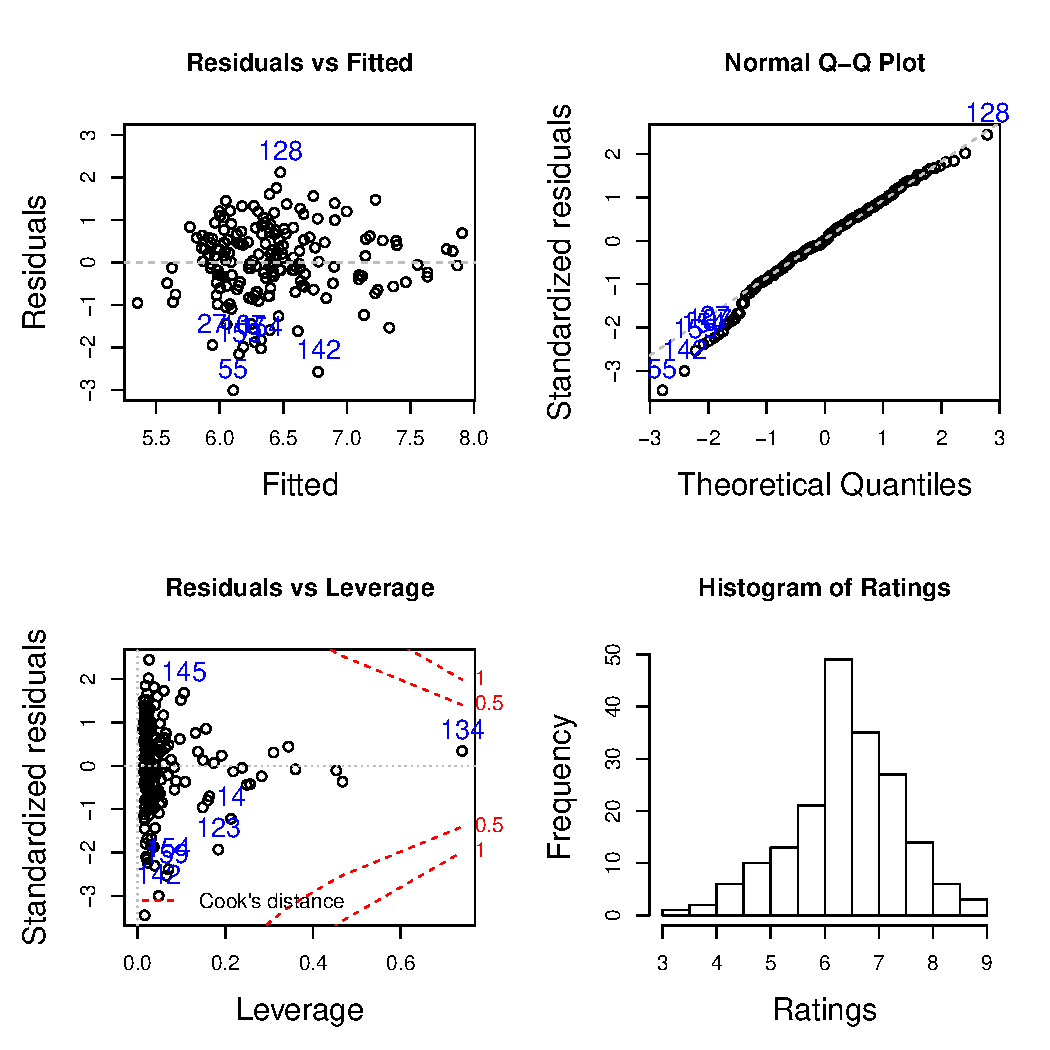
\includegraphics[width = \textwidth]{figure1.pdf}
\caption{\label{fig:csm_Figure1} Diagnostic plots of CSM data. Plots at the top left, top right and bottom left were obtained with \code{plot.kspm}. They represent respectively residuals against fitted values, the normal Q-Q plot of residuals and residuals against leverage with the Cook's distance information. Plot at the bottom right represents the distribution of ratings in the database.}
\end{figure}

Outlier points are annotated and we can see movie $134$ (\textit{Jurassic World}) has high leverage. Also of note, the lower tail of the residuals distribution is not as expected for a Normal distribution. The histogram of ratings shows that the deviation could be due to the left skewed distribution of the response variable. 



The derivative function may help to interpret the effect of each variable individually on the outcome. Indeed, the sign of the derivatives captures variational changes of the effect of the variable on the outcome. To illustrate this feature, Figure~\ref{fig:csm_Figure2} displays the derivatives for Gross income, Budget and Screens. It has been generated with the following code:


\begin{example}
> par(mfrow = c(1,2), mar = c(5,5,5,2))
> plot(derivatives(csm.fit1), subset = "Gross", cex.lab = 1.5, cex = 1.3,
+    main = "Pointwise derivatives according to Gross Income")
> plot(derivatives(csm.fit1), subset = "Screens", col = csm$Sequel,
+    cex.lab = 1.5, cex = 1.3, pch = 16, main = "Pointwise derivatives
+    according to Number of Screens \n and Sequel")
> legend("topleft", fill = palette()[1:7], legend = 1:7, title = "Sequel", 
+    horiz = TRUE)
\end{example}


\begin{figure}[htbp]
\centering
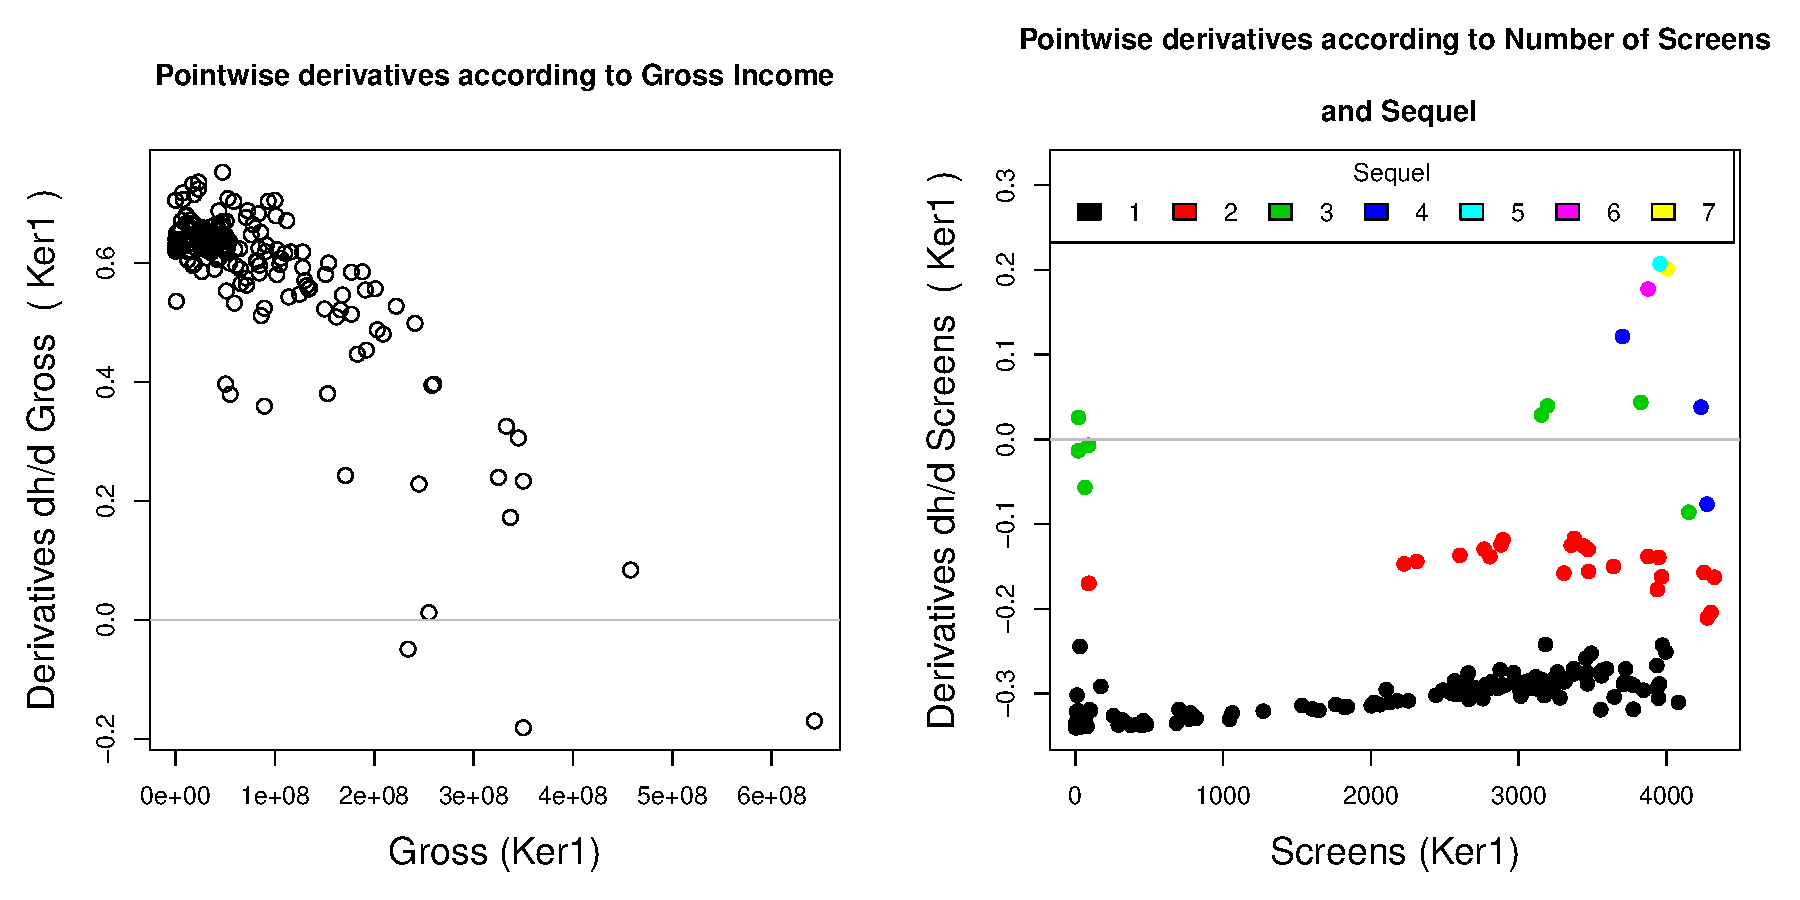
\includegraphics[width = \textwidth]{figure2.pdf}
\caption{\label{fig:csm_Figure2} Derivative plots on CSM data obtained with \code{plot.derivatives}. Each point corresponds to an observation. Plot on the left represents the pointwise derivatives according to the Gross income variable. Plot on the right represents the pointwise derivatives according to the Screens variable and are colored according Sequel variable showing a probable interaction between Screens and Sequel.}
\end{figure}

By default, the X-axis label gives the name of the variable and, in brackets, the kernel in which it is included. When only one kernel is included in the kernel, it is named \code{Ker1}. Because genre and sequel variables, even if they are numeric, refer to categorical variables, it is possible to easily highlight some patterns of interaction between these variables and the others. Derivatives according to Gross income are mostly positive meaning that higher Gross income is associated with higher ratings. However the slope of this effect decreases as the gross income grows. It is difficult to interpret the derivatives for Gross income higher than 2.5e+08 since this category includes only a few movies. Based on the display in the right panel, whether a movie has sequels seems to interact with the effect of the number of screens on the ratings. Indeed when the movie is the first or second release (Sequel = 1 or 2), the derivatives are always negative meaning that as the number of screens on which the movie is released increases, the ratings tend to decrease. However, this relationship seems to be stronger for the first release than the second. No clear pattern can be observed for subsequent sequels. It is difficult to know if this reveals an absence of effect or whether there are simply too few movies past sequel $2$ in these data. 





To help in the choice of the kernel function, we may compare several models by using information criteria. As an example, we fit a second model assuming a polynomial kernel function with fixed tuning parameters ($\rho=1$, $\gamma=1$ and $d=2$). This model can be compared to the previous one using information criteria such as the AIC or BIC. By default the \code{extractAIC()} command gives the AIC.


\begin{example}
> csm.fit2 <- kspm(response = "Ratings", kernel = ~Kernel(~Gross + Budget +
+    Screens + Sequel, kernel.function = "polynomial", rho = 1, gamma = 1,
+    d = 2), data = csm, level = 0)
> extractAIC(csm.fit1)
\end{example}
\begin{example}
[1] 941.4521
\end{example}
\begin{example}
> extractAIC(csm.fit2)
\end{example}
\begin{example}
[1] 944.4618
\end{example}


Here, we concluded that gaussian kernel function fits our data better than the polynomial kernel function, given the tuning parameters we considered.

\subsubsection{Adding social media features to the model: a model with kernel interaction} \label{sec:illustrations-csm-model2}

Now, we assume a model with two kernel parts, one for conventional features and one for social media features, as well as their interaction. We propose to use the gaussian kernel function for each set of features, although different kernels could be used. The hyperparameters we chose are those obtained for each kernel separately.


\begin{example}
> csm.fit3 <- kspm(response = "Ratings", linear = NULL, kernel = ~Kernel(~ 
+    Gross + Budget + Screens + Sequel, kernel.function = "gaussian",
+    rho = 61.22) * Kernel(~ Sentiment + Views + Likes + Dislikes + Comments + 
+    Aggregate.Followers, kernel.function = "gaussian", rho = 1.562652),
+    data = csm)
\end{example}


While the model is running, R returns a summary of the kernel part(s) and interaction(s) included in the model.


\begin{example}
------------------------------------------------------------------ 
The model includes the following kernels:  
Ker1 
Ker2 
Ker1:Ker2
------------------------------------------------------------------ 
Details: 
Ker1: ~Kernel(~Genre + Gross + Budget + Screens + Sequel,
kernel.function = "gaussian", rho = 55.5897)
Ker2: ~Kernel(~Sentiment + Views + Likes + Dislikes + Comments +
Aggregate.Followers, kernel.function = "gaussian", rho = 1.562652)
------------------------------------------------------------------
\end{example}


As defined by model~(\ref{eq:inter}), the \code{summary()} command will return the $p$~value of tests $H_0: h_1(.) = 0$, $H_0: h_2(.) = 0$ and $H_0: h_{12}(.) = 0$. By default all tests are performed. However, if our interest lies only in the test of interaction, the \code{kernel.test} option may be used to choose the test of interest and reduce the computation time. If interest lies in the global test $H_0: h_1(.) = h_2(.) = h_{12}(.) = 0$, the \code{global.test} option should be set at \code{TRUE}.


\begin{example}
> summary(csm.fit3, kernel.test = "Ker1:Ker2", global.test = TRUE)
\end{example}
\begin{example}
Call:
kspm(response = "Ratings", linear = NULL, kernel = ~Kernel(~Gross + 
    Budget + Screens + Sequel, kernel.function = "gaussian", 
    rho = 61.22) * Kernel(~Sentiment + Views + Likes + Dislikes + 
    Comments + Aggregate.Followers, kernel.function = "gaussian", 
    rho = 1.562652), data = csm)

Sample size:
n = 187

Residuals: 
    Min      Q1  Median      Q3     Max 
-1.4185 -0.3396  0.0112  0.3291  1.3597 

Coefficients (linear part): 
            Estimate Std. Error  t value     Pr(>|t|)
(Intercept) 4.548524   1.256813 3.619095 0.0004324838

Score test for non-parametric kernel: 
          lambda        tau   p-value
Ker1:Ker2    187 0.00208359 0.7376828

Global test: p-value = 6e-04

Residual standard error: 0.62 on 121.17 effective degrees of freedom
Multiple R-squared: 0.7452, Adjusted R-squared: 0.6089
\end{example}


Adding social media features to the model improved the predictions as indicated by the adjusted $R^2$. However the smooth function associated with the kernel interaction does not significantly differ from the null, leading to the conclusion that there is no interaction effect between conventional and social media features on the ratings. 



Suppose now, we want to predict the ratings that will be attributed to the three artificial movies described in tables~\ref{table:csm-predict1} and~\ref{table:csm-predict2} below, according to the model \code{csm.fit3}.

\begin{table}[htbp]
\centering
\begin{tabular}{rrrrr}
\toprule
& Gross & Budget & Screens & Sequel  \\
\midrule
Movie 1 & 5.0e+07 & 1.8e+08 &   3600    &  2   \\
Movie 2 & 50000 & 5.2e+05  &   210  &    1    \\
Movie 3 & 10000 & 1.3e+03   & 5050  &    1   \\
 \bottomrule
\end{tabular}
\caption{\label{table:csm-predict1} The conventional features of three artificial movies. Rows represent the new movies and columns represent the features.}
\end{table}

\begin{table}[htbp]
\centering
\begin{tabular}{rrrrrrr}
\toprule
& Sentiment &  Views & Likes & Dislikes & Comments  & Aggregate.Followers \\
\midrule
Movie 1 &  1 & 293021 & 3698 & 768  &     336   &           4530000 \\
Movie 2 &  2 &  7206 &  2047 &    49    &    70        &       350000 \\
Movie 3 &  10 & 5692061 &  5025 & 305  &     150         &      960000 \\
 \bottomrule
\end{tabular}
\caption{\label{table:csm-predict2} The social media features of three artificial movies. Rows represent the new movies and columns represent the features.}
\end{table}



\begin{example}
> newdata.Ker1 <- data.frame(Gross = c(5.0e+07, 50000, 10000), 
+    Budget = c(1.8e+08, 5.2e+05, 1.3e+03), Screens = c(3600, 210, 5050), 
+    Sequel = c(2, 1, 1))
> newdata.Ker2 <- data.frame(Sentiment = c(1, 2, 10), Views = c(293021,
+    7206, 5692061), Likes = c(3698, 2047, 5025), Dislikes = c(768, 49,
+    305), Comments = c(336, 70, 150), Aggregate.Followers = c(4530000,
+    350000, 960000))
> predict(csm.fit3, newdata.kernel = list(Ker1 = newdata.Ker1, Ker2 =
+    newdata.Ker2), interval = "prediction")
\end{example}
\begin{example}
       fit      lwr      upr
1 4.682560 3.147755 6.217365
2 6.401853 5.100309 7.703396
3 6.128641 4.395417 7.861864
\end{example}


The output of the \code{predict()} function gives the predicted values (\code{fit}) and the lower (\code{lwr}) and upper (\code{upr}) bounds of prediction intervals.

We may obtain the predictions for the original data directly from the model or from the \code{predict()} function. With the latter, confidence intervals may be additionally obtained.


\begin{example}
> pred <- csm.fit3$fitted.value
> pred <- predict(csm.fit3, interval = "confidence")
> plot(csm$Ratings, pred$fit, xlim = c(2, 10), ylim = c(2, 10), 
+    xlab = "Observed ratings", ylab = "Predicted ratings", cex.lab = 1.3)
> abline(a = 0, b = 1, col = "red", lty = 2)
\end{example}


\begin{figure}[htbp]
\centering
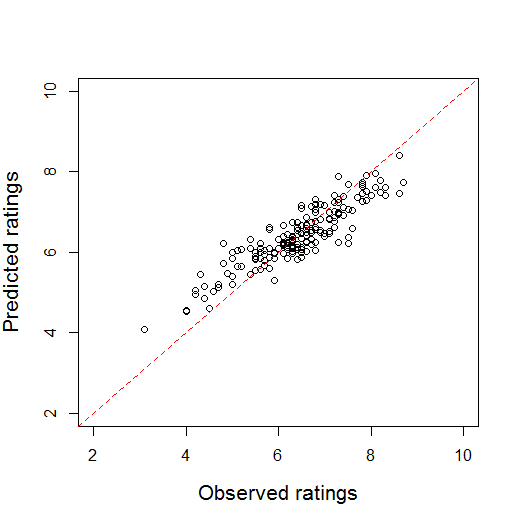
\includegraphics[width = 7cm]{figure3}
\caption{\label{fig:csm_Figure3} Predicted versus observed ratings in CSM dataset. Red dotted line represents a perfect concordance between predictions and observations.}
\end{figure}

Figure~(\ref{fig:csm_Figure3}) shows that for smaller values, the model overestimates the outcome. This is again probably due to the left skewness of the outcome distribution.

\subsubsection{An example of the variable selection procedure} \label{sec:illustrations-csm-model3}

Suppose we fit a single kernel semi-parametric model with a gaussian kernel to adjust the social media features in the CSM data. The kernel part contains the set of social media features. We want to select the relevant variables to be included in the kernel. We therefore can perform a stepwise variable selection procedure based on AIC, while letting $\rho$ vary at each iteration. To do so, we first fit the full model including all features.


\begin{example}
> csm.fit4 <- kspm(response = "Ratings", kernel = ~Kernel(~ Sentiment + Views  
+    + Likes + Dislikes + Comments + Aggregate.Followers, kernel.function = 
+    "gaussian"), data = csm)
\end{example}


Then, we apply the \code{stepKSPM()} command on the full model as follows.


\begin{example}
> stepKSPM(csm.fit4, kernel.lower = ~1, kernel.upper = ~ Sentiment + Views 
+    + Likes + Dislikes + Comments + Aggregate.Followers, direction = "both", 
+    k = 2, kernel.param = "change", data = csm)
\end{example}


At each iteration, R returns the current model, and the list of variables that may be added or removed.


\begin{example}
Start: AIC = 913.2
Linear part: ~ 1
Kernel part: ~ Sentiment + Views + Likes + Dislikes + Comments +
               Aggregate.Followers

                        Part      AIC
- Sentiment           kernel 910.8282
<none>                       913.1769
- Views               kernel 913.9753
- Likes               kernel 917.6532
- Comments            kernel 921.2163
- Aggregate.Followers kernel 925.4491
- Dislikes            kernel 969.4304


Step: AIC = 910.8
Linear part: ~ 1
Kernel part: ~ Views + Likes + Dislikes + Comments + Aggregate.Followers

                        Part      AIC
- Views               kernel 905.2908
<none>                       910.8282
+ Sentiment           kernel 913.1769
- Aggregate.Followers kernel 915.5481
- Likes               kernel 916.8125
- Comments            kernel 921.9627
- Dislikes            kernel 970.3804


Step: AIC = 905.3
Linear part: ~ 1
Kernel part: ~ Likes + Dislikes + Comments + Aggregate.Followers

                        Part      AIC
<none>                       905.2908
+ Views               kernel 910.8282
+ Sentiment           kernel 913.9753
- Aggregate.Followers kernel 916.0224
- Comments            kernel 917.8758
- Likes               kernel 925.0230
- Dislikes            kernel 968.2502
\end{example}


The final model includes the variables \code{Likes}, \code{Dislikes}, \code{Comments} and \code{Aggregate.Followers}. 



\section{Example 2: Consumption of energy data} \label{sec:illustrations-energy}
Our second example illustrates how \pkg{KSPM} may be efficient with complex data as time series and show how the choice of tuning parameters impacts the results.

The \code{energy} data is a set of data on energy consumption each hour on Ouessant island (France) from September the 13th, 2015 to October the 4th, 2015, that were made publicly available by \textit{Electricit\'e de France} at https://iles-ponant-edf-sei.opendatasoft.com. The data set also contains corresponding meteorologic data such as temperature (Celsius degrees), pressure (Pa) and humidity rate (g/m$^3$). These measures are collected by \textit{Meteo France} every 3 hours and are publicly available on www.infoclimat.fr. We obtained hourly values by linear interpolation. In total the data set contains 504 measurements.


\begin{example}
> data("energy")
> head(energy)
\end{example}
\begin{example}
     power       date        T        P       HR hour hour.num
1 526.1667 2015-09-13 12.43333 1007.933 81.66667  01h        1
2 495.0000 2015-09-13 12.36667 1007.167 82.33333  02h        2
3 446.1667 2015-09-13 12.30000 1006.400 83.00000  03h        3
4 365.8333 2015-09-13 12.30000 1005.833 82.66667  04h        4
5 341.0000 2015-09-13 12.30000 1005.267 82.33333  05h        5
6 352.3333 2015-09-13 12.30000 1004.700 82.00000  06h        6
\end{example}


These data demonstrate strong periodicity depending on time of day (Figure~\ref{fig:energy_Figure1}). Of note, if data had been collected for a period longer than one year, a second periodicity would be visible corresponding to seasons.


\begin{figure}[htbp]
\centering
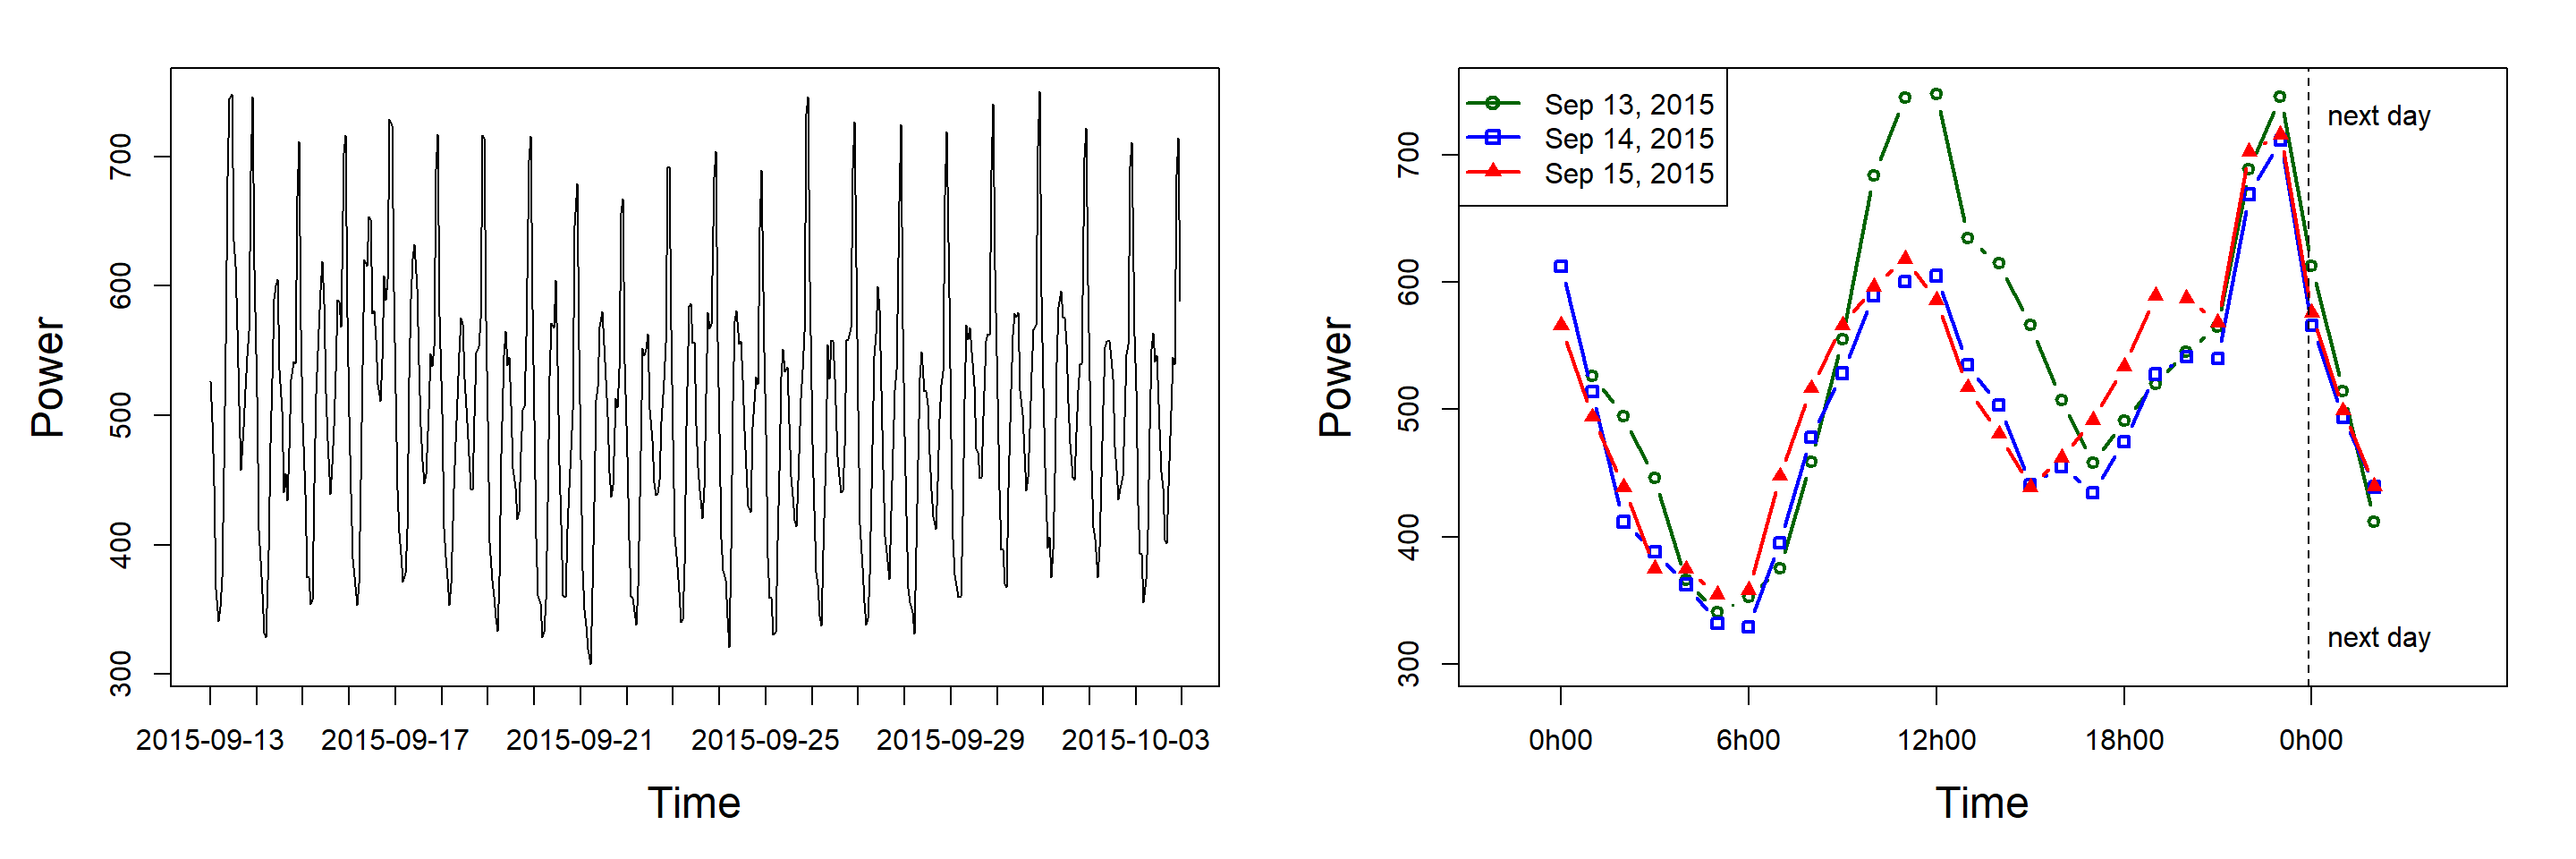
\includegraphics[width=\textwidth]{figure4}
\caption{\label{fig:energy_Figure1} Pattern of energy consumption over the entire data set from Ouessant island (Left) and on the three first days (Right). The power is observed each hour and show a one day periodicity.} 
\end{figure}

We will consider the 408 first measurements (17 days) as the training set. The others 4 days will be used as a test set, where we want to predict the energy consumption. 


\begin{example}
> energy_train_ <- energy[1:408, ]
> energy_test_ <- energy[409:504, ]
\end{example}


\subsubsection{Modeling} \label{sec:illustrations-energy-model1}

We fit a single kernel semi-parametric model to the training data. We assume that energy depends linearly on temperature (\code{T}), and therefore this variable is included in the linear part of the model. The other meteorologic data, as well as hours in 24-hour numeric format, are included in the kernel part of the model. We used a gaussian kernel and we left the $\rho$ parameter free to be estimated by the model. 


\begin{example}
> energy.fit1 <- kspm(response = "power", linear = ~T, kernel = ~Kernel(~
+    hour.num + P + HR, kernel.function = "gaussian") , data = energy_train_)
> energy.fit1$kernel.info$Ker1$rho
\end{example}
\begin{example}
     par1 
0.7028723 
\end{example}


\subsubsection[Impact of the rho parameter on derivatives and predictions]{Impact of the $\rho$ parameter on derivatives and predictions} \label{sec:illustrations-energy-impact_rho}

We recomputed the model using other values for the $\rho$ parameter to explore sensitivity of the results to this key kernel parameter. Values were chosen tenfold larger and smaller than the estimated value of $0.70$ in \code{energy.fit1}.


\begin{example}
> energy.fit2 <- kspm(response = "power", linear = ~T, kernel = ~Kernel(~
+    hour.num + P + HR, kernel.function = "gaussian", rho = 7) , data =
+    energy_train_)
> energy.fit3 <- kspm(response = "power", linear = ~T, kernel = ~Kernel(~
+    hour.num +  P + HR, kernel.function = "gaussian", rho = 0.07) , data = 
+    energy_train_)
\end{example}


Figure~\ref{fig:energy_Figure2} displays the predictions obtained on both the training and test data sets, as well as the derivatives, as a function of the hours variable, for the three models \code{energy.fit1}, \code{energy.fit2} and \code{energy.fit3} that differ only on the value of the tuning parameter $\rho$. 


\begin{figure}[htbp]
\centering
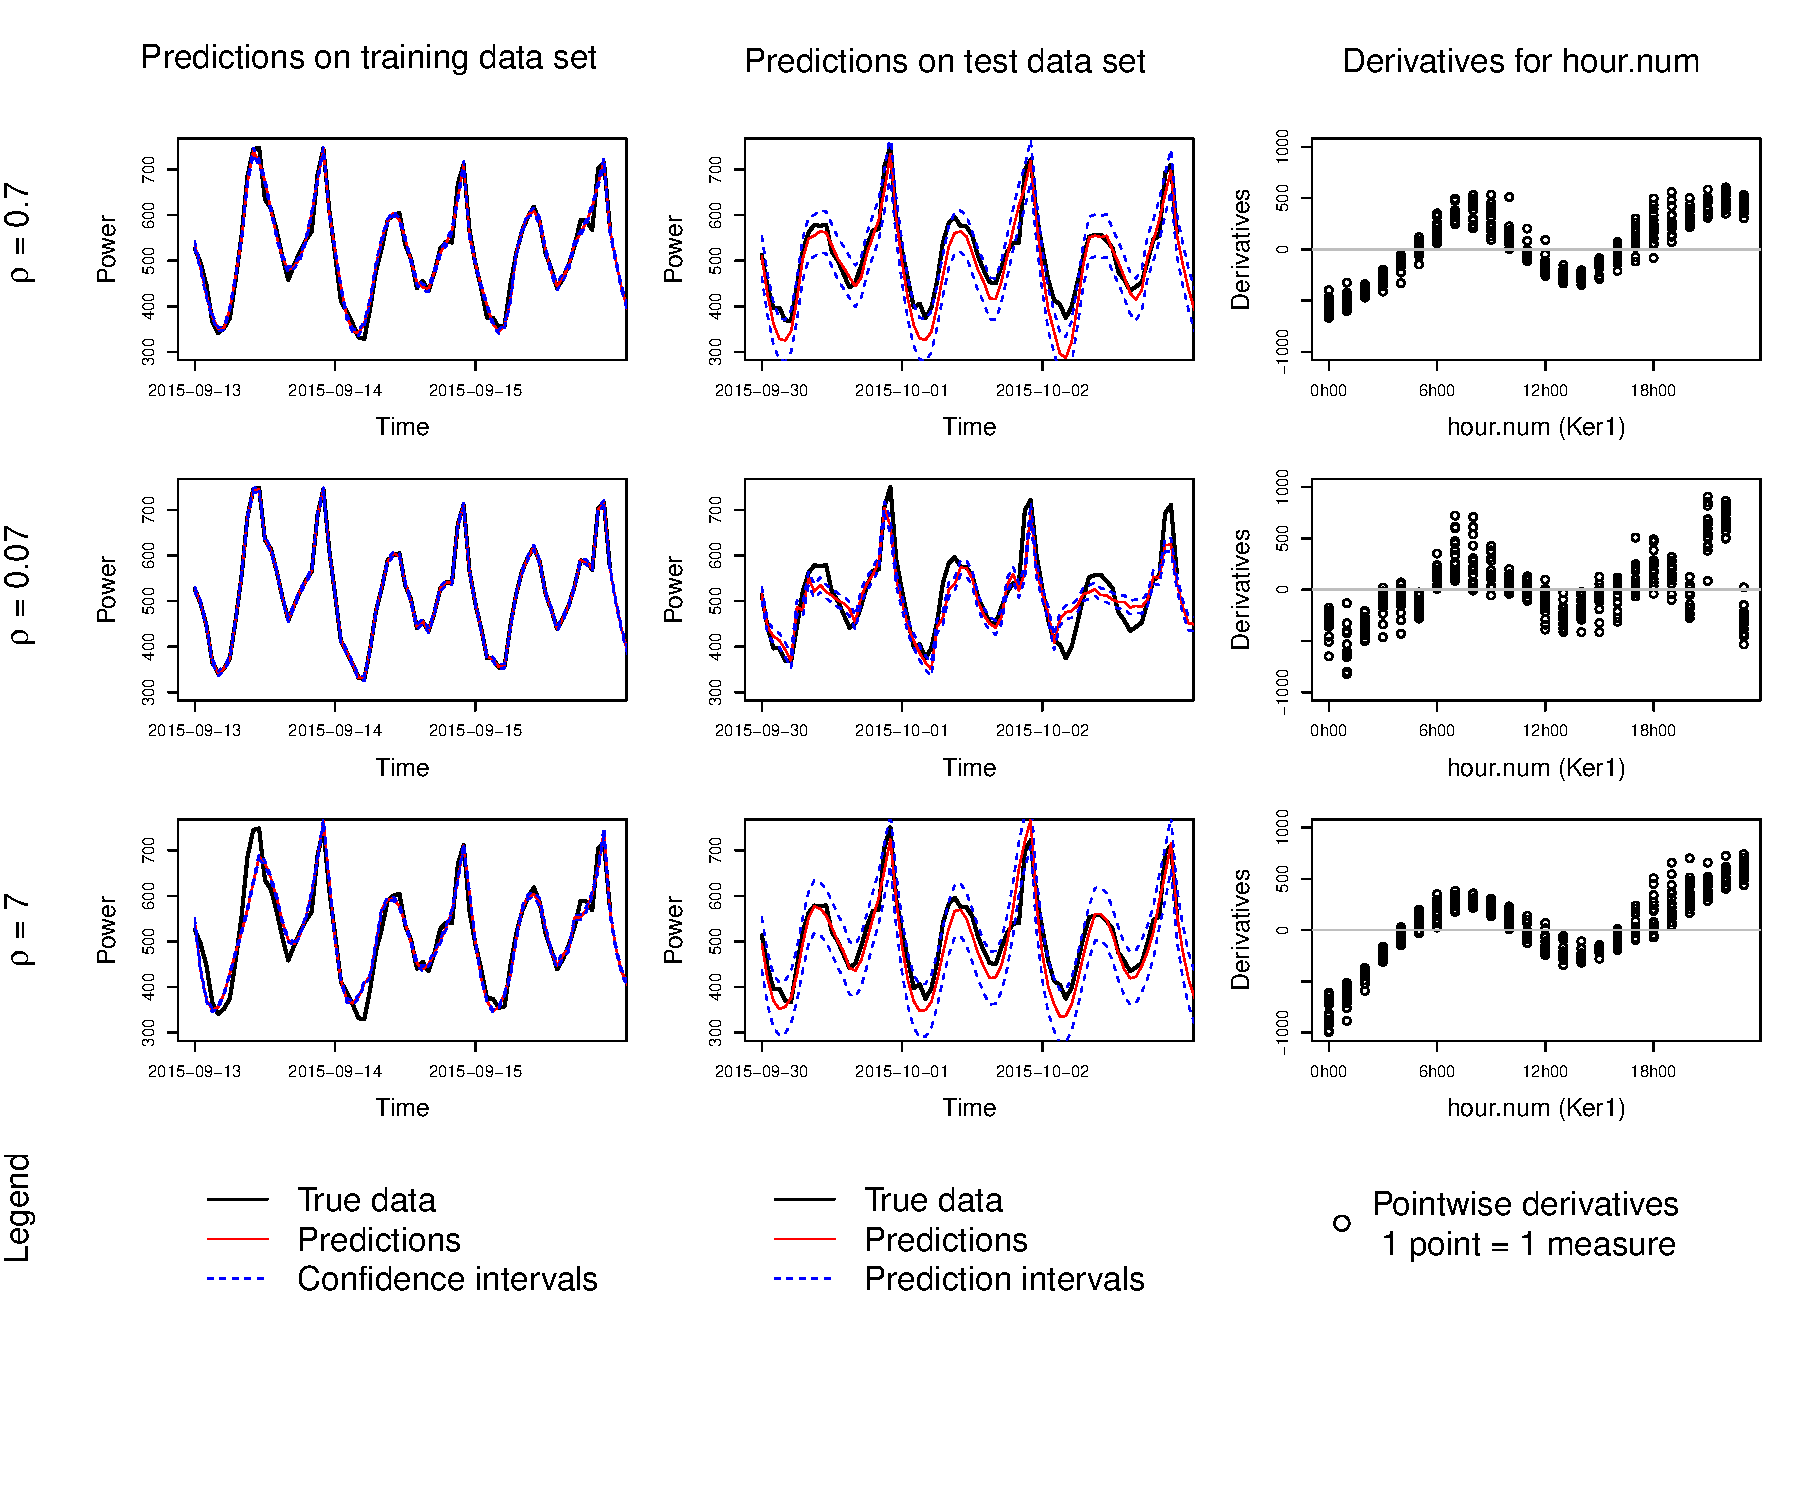
\includegraphics[width=\textwidth,  trim = 0cm 3cm 0cm 0cm, clip]{figure5}
\caption{\label{fig:energy_Figure2} Predictions and derivatives obtained for different values of $\rho$ in the energy dataset. Predictions on training data set are displayed with confidence intervals, whereas predictions on test data set are displayed with prediction intervals. The first row corresponds to the model \code{energy.fit1} with estimated $\rho=0.7$. The second row corresponds to a tenfold smaller $\rho=0.07$ (overfitting) and third row corresponds to a tenfold larger $\rho=7$ (underfitting). The last column shows how the choice of $\rho$ impacts the derivatives.}
\end{figure}


The first row of Figure~\ref{fig:energy_Figure2} corresponds to the model with the value of $\rho$ estimated by the model. Predictions fit well for both the training and the test sets. The derivative graph shows that between 6h00 and 12h00 and between 18h00 and 23h00 the derivatives are positive. This result is coherent with the increase of energy consumption during these times of the day (Figure~\ref{fig:energy_Figure1}-Right). Inversely between 0h00 and 6h00 and between 12h00 and 18h00, the energy consumption decreases as showed by negative values of derivatives. One might have expected that derivative values should be close between 0h00 and 23h00 but the peak consumption observed at 23h00 everyday (Figure~\ref{fig:energy_Figure1}) is probably associated with a sudden change in derivative values that is difficult to smooth accurately.



This example shows how a gaussian kernel function may handle complex functional data. However the choice of the $\rho$ parameter may influence the results. A higher $\rho$ leads to a smoother approximation of $h(.)$ and worsens the predictions. Indeed, a higher $\rho$ may perfectly fit the training data set, but this corresponds to a case of model overfitting, which results in biased predictions in the test set. In contrast, a lower $\rho$ may lead to underfitting of training and test data sets. The choice of the $\rho$ parameter also impacts the derivatives; indeed a higher $\rho$ induces more noise among the derivatives.



\section{Example 3: Gene-gene interaction} \label{sec:illustrations-gene}
This example shows how the interaction test may be applied to gene-gene interaction using standard linear kernel and SNPs involved in genes.

We simulated a data of 300 subjects and 9 SNPs, 6 belonging to gene A and 3 belonging to gene B, using the \code{glSim()} function into the \CRANpkg{adegenet} R package~\citep{adegenet}. SNPs are coded 0, 1 or 2 according to the number of alleles of each type carried by the subject.
A continuous outcome was simulated as a linear combination of the interaction terms between the 6 SNPs of gene A and the three SNPs of gene B, where the weight coefficients where randomly and uniformly chosen in the interval $\left[-2;0\right]$. We added an intercept of 100 and a normally distributed error of mean 0 and standard deviation 15. Code details are available in Supplement S1.


Let \code{y} be the vector of continuous outcomes, \code{geneA} be the $300 \times 6$ matrix of SNPs belonging to gene A and \code{geneB} be the $300 \times 3$ matrix of SNPs belonging to gene B. 



We test the interaction between the genes using the code below. Of note, in this example, the data are specified using vector and design matrices instead of using formulae and data frame as in previous examples.



\begin{example}
> gene.fit <- kspm(response = y, kernel = ~ Kernel(geneA, kernel = "linear") 
+    * Kernel(geneB, kernel = "linear"))
> summary(gene.fit, kernel.test = "Ker1:Ker2")
\end{example}
\begin{example}
Call:
kspm(response = y, kernel = ~Kernel(geneA, kernel = "linear") * 
    Kernel(geneB, kernel = "linear"))

Sample size:
n = 300

Residuals: 
     Min       Q1   Median       Q3      Max 
-34.1111  -8.7300  -1.1659   9.7299  38.6887 

Coefficients (linear part): 
            Estimate Std. Error  t value      Pr(>|t|)
(Intercept) 88.80183  0.8178659 108.5775 2.531469e-231

Score test for non-parametric kernel: 
            lambda       tau     p-value
Ker1:Ker2 199.4587 0.9862838 0.006646781

Residual standard error: 14.03 on 280.74 effective degrees of freedom
Multiple R-squared: 0.2387, Adjusted R-squared: 0.1892
\end{example}


The result suggests that genes A and B impact the continuous outcome y through their interaction.

%\section{Another section}

%There will likely be several sections, perhaps including code snippets, such as:

%\begin{example}
%  x <- 1:10
%  result <- myFunction(x)
%\end{example}

\section{Summary}

%This file is only a basic article template. For full details of \emph{The R Journal} style and information on how to prepare your article for submission, see the \href{https://journal.r-project.org/share/author-guide.pdf}{Instructions for Authors}.

This new \pkg{KSPM} package provides a flexible implementation of the kernel semi-parametric model and its extensions in a unified framework, using nomenclatures similar to other regression R packages. Thanks to the kernel trick, such a model is useful when interest lies in prediction and our \code{predict()} command makes this easy. Nevertheless, inference is also possible through the confidence intervals and tests provided by the package, such as through the \code{summary()} command. Moreover, we have provided many options for model diagnostics (residuals,  leverage, ...), model interpretation (derivatives, ...) and model comparisons (AIC, stepwise, ...).\\

Model estimation for multiple kernel model is based on an iterative estimation of regression parameters we develop and prove in Supplement S2. Penalization and tuning parameter estimation involves \code{optimize()} and \code{DEoptim()} functions. The both integrate C code ensuring a faster convergence of the algorithms. However, the overall \pkg{KSPM} algorithm includes inversion of $n \times n$ matrices, thereby resulting in slower optimization as $n$ increases. It would improve \pkg{KSPM}'s performance to combine matrix inversion code and optimization code in a single efficient set of C code and we are considering this for a future implementation.  It is worth noting, however, that computation time is not severely impacted by the number of predictors even if $n << q$.



In the \pkg{KRLS} package, \cite{hainmueller2013kernel} proposed a marginal test for the individual effect of each variable included in the kernel. We decided not to implement this test in our package since the marginal effect may mask interesting but symmetric effects of a variable on the continuous outcome. However, we have implemented a test of hypothesis based on variance components to test the joint effect of a set of variables on the continuous outcome. The distribution of this test statistic follows a mixture of $\chi^2$ distributions that we approximated using Davies' method~\citep{davies1980distribution}, available through the \CRANpkg{CompQuadForm} package~\citep{CQFpackage, compQuadForm}. The distribution can also be approximated by a scaled chi-squared distribution using Satterthwaite's method where parameters are computed by moment matching. \cite{schifano2012snp} compared the two approximation methods on the type-I error rate in a single kernel semi-parametric model and showed that the rate is inflated with Satterthwaite's method when the $\alpha$-level is low, and therefore we recommend the Davies method. To assess global testing of multiple kernels, we implemented a sum of the L single-kernel test statistics as an overall test statistic. In general, the computation of the $p$~value of this overall test involves the joint distribution of ($Q_1$, ... $Q_L$). To derive analytical values for the overall $p$~value, one can use techniques similar to those used in~\cite{sun2018}, which relied on a copula-based model to approximate this joint distribution. This last option is not yet implemented in \pkg{KSPM}.



For all our tests, the model has to be re-estimated under the null hypothesis for the kernel of interest. If the resulting null model still contains one or more kernel part(s), we made the choice to recompute penalization parameter(s), since this choice ensures an optimized model under the null hypothesis. However, we have also decided to leave the kernel tuning parameters fixed when re-estimating under the null. Indeed, a change in tuning parameters induces a change in the choice of kernel functions - and thus in model assumptions - and hence, keeping the tuning parameters fixed ensures comparability of model assumptions under the null and the alternative hypotheses. 

In our \pkg{KSPM} package, we have also included an algorithm for selection of variables based on these information criteria. Backward, forward or stepwise approaches can be chosen for single kernel semi-parametric models. Although these concepts may be easily extended to the case of multiple kernel models, such analyses require large computing times. Parallelization of such a process may greatly increase the appeal of this  procedure. For now, we recommend investigating variables within a single kernel before starting to fit multiple kernel models. 

In summary, the \pkg{KSPM} package is a flexible comprehensible option for studying the effects of groups of variables on a continuous outcome. These tools may be extended to the case of binary or survival outcomes in future work. 


\section{Acknowledgements}

CS  was  supported  by  the  Institute  for  Data  Valorization  (IVADO)  fellowship. CG was supported by the Ludmer Centre for Neuroinformatics and Mental Health, the Canadian Institutes for Health Research, as well as the CIHR PJT 148620 grant. SJ is a recipient of a Canada Research Chair in neurodevelopmental disorders, and a chair from the Jeanne et Jean Louis Levesque Foundation. This research was enabled in part by support provided by Calcul Quebec (http://www.calculquebec.ca) and Compute Canada (www.computecanada.ca). This work is supported by a grant from the Brain Canada Multi-Investigator initiative and CIHR grant 159734 (SJ, CMTG).  This work was also supported by an NIH award U01 MH119690 granted (SJ) and U01 MH119739.

\bibliography{schramm}

\newpage

\begin{center}
    \textbf{SUPPLEMENT}
\end{center}

\section{Supplement S1}

We simulated a $300 \times 9$ matrix representing the number of minor allele (0, 1 or 2) of 300 subjects for 9 SNPs, 6 belonging to gene A and 3 belonging to gene B, using the \code{glSim()} function into the \pkg{adegenet} R package. 

\begin{example}
> library(adegenet)
> set.seed(78)
> SNPdata <- as.matrix(glSim(n.ind = 300, n.snp.nonstruc = 9, n.snp.struc = 0, k = 1,
  LD = FALSE, ploidy = 2))
\end{example}

\noindent We may deduce two matrices, one with data belonging to gene A and one with data belonging to gene B.

\begin{example}
> geneA <- SNPdata[,1:6]
> geneB <- SNPdata[,7:9]
\end{example}

\noindent Then we computed the matrix of interactions between SNPs from gene A and SNPs from geneB.

\begin{example}
> SNPdataAB <- matrix(NA, nrow = 300, ncol = 6*3)
> k <- 1
> for (i in 1:6) {
    for (j in 1:3) {
      SNPdataAB[,k] <- SNPdataA[,i] * SNPdataB[,j]
      k <- k+1
    }
  }
\end{example}

A continuous outcome was simulated as a linear combination of the interaction terms between the 6 SNPs of gene A and the three SNPs of gene B, where the weight coefficients where randomly and uniformly chosen in the interval $\left[-2;0\right]$ using the following code.

\begin{example}
> beta <- as.matrix(runif(6*3,-2,0), nrow = 300)
> y <- 100 + SNPdataAB %*% beta + rnorm(n, 0, 15)
\end{example}

\noindent Of note, we added an intercept of 100 and a normally distributed error of mean 0 and standard deviation 15.


\section{Supplement S2}

\noindent Estimating the kernel semi-parametric model parameters consists in estimating $\alpha_1, ..., \alpha_L$ and $\beta$. Then, estimators of $h_1(.)$, ..., $h_L(.)$ are deduced from $\hat{\alpha}_1, ..., \hat{\alpha}_L$. When there are multiple kernels, estimation is iterative and so we proceed as follows. Partial derivatives of $l(\beta, h)$ according to $\alpha_1, ..., \alpha_L$ and $\beta$ lead to the following equations: 

\begin{equation}\label{eq:betaM}
\hat{\beta} =  \left\lbrace X^\top \left( I - \sum\limits_{\ell = 1}^L K_{\ell} G_{\ell}^{-1} M_{\ell} \right) X  \right\rbrace^{-1}  X^\top \left(I - \sum\limits_{\ell = 1}^L K_{\ell} G_{\ell}^{-1} M_{\ell}\right) Y
\end{equation}
\begin{equation}\label{eq:alphaM}
\forall \ell \in \left\lbrace 1,..., L\right\rbrace, \quad \hat{\alpha}_{\ell} =  G_{\ell}^{-1} M_{\ell} \left(Y-X\hat{\beta}\right)
\end{equation}
where $I$ is the $n \times n$ identity matrix and $\forall \ell \in \left\lbrace 1, ..., L \right\rbrace$, $G_{\ell}$ and $M_{\ell}$ are computed using an iterative process as described below:
\begin{itemize}
    \item Re-order elements $\alpha_{1...L}$, $K_{1...L}$ and $\lambda_{1...L}$ such that the last is the $\ell^{th}$ element
    \item Note $\alpha_{(1)}$, ..., $\alpha_{(L)}$, $K_{(1)}$, ..., $K_{(L)}$ and $\lambda_{(1)}$, ..., $\lambda_{(L)}$ the re-ordered elements with $\alpha_{(L)} = \alpha_{\ell}$, $K_{(L)} = K_{\ell}$ and $\lambda_{(L)} = \lambda_{\ell}$
    \item Define iteratively $\mathcal{M}_{(0)...(L)}$ and $\mathcal{G}_{(1)...(L)}$ by $\mathcal{M}_{(0)} = I$ the $n \times n$ identity matrix and $\forall m \in \left\lbrace 1, ..., L \right\rbrace$: \\
    $\mathcal{G}_{(m)} = \lambda_{(m)} I + \mathcal{M}_{(m-1)} K_{(m)}$ \\
    $\mathcal{M}_{(m)} = \left(I - \mathcal{M}_{(m-1)} K_{(m)} \mathcal{G}_{(m)}^{-1} \right) \mathcal{M}_{(m-1)}$
    \item Compute $G_{\ell}$ and $M_{\ell}$ as:\\
$G_{\ell} = \mathcal{G}_{(L)}$ \\
$M_{\ell} = \mathcal{M}_{(L-1)}$
\end{itemize}


\noindent Whereas the parameter estimation for single kernel model has been largely demonstrated, the equations for computing multiple kernel parameters were not theoretically developed yet. Above, we propose an iterative way to estimate the parameters for all kernel models. Below, we propose the proof for equations (\ref{eq:betaM}) and (\ref{eq:alphaM}).\\

\noindent \textbf{\underline{Proof:}} \\

\begin{changebar}[0.2cm]
\noindent Partial derivatives of penalized likelihood~(\ref{eq:pll}) lead to equations below:


\begin{equation} \label{eq:derivll}
\left\lbrace \begin{aligned}
X^\top (Y - X\beta - \sum\limits_{\ell = 1}^L K_{\ell} \alpha_{\ell}) & =  0 \\
Y - X\beta - \sum\limits_{m = 1}^L K_{m} \alpha_{m} - \lambda_{\ell} \alpha_{\ell} & =  0 \quad \forall \ell \in \left\lbrace 1,...,L \right\rbrace
\end{aligned} \right.
\end{equation}


\noindent \textit{Proposition 1:} $\forall k \in \left\lbrace 1, ..., L-1\right\rbrace, \alpha_{(k)} = \mathcal{G}_{(k)}^{-1} \mathcal{M}_{(k - 1)} \left( Y - X\beta - \sum\limits_{m = k + 1}^L K_{(m)} \alpha_{(m)} \right)$ \\

\noindent \textit{Proposition 2:} if proposition 1 is true until $k$, then 
$$\sum\limits_{j = 1}^k K_{(m)}\alpha_{(m)} = (I - \mathcal{M}_{(k)})\left( Y - X\beta - \sum\limits_{m = k + 1}^L K_{(m)}\alpha_{(m)} \right)$$

\noindent \textit{(Proofs of propositions 1 and 2 are given below.)} \\

\noindent Now, suppose proposition 1 and proposition 2 are true.

\begin{align*}
(\ref{eq:derivll}) \Rightarrow && Y - X\beta - \sum\limits_{m = 1}^L K_{(m)}\alpha_{(m)} - \lambda_{(L)}\alpha_{(L)} &= 0  \\
\Leftrightarrow &&  Y - X\beta - \sum\limits_{m = 1}^{L-1} K_{(m)}\alpha_{(m)} - K_{(L)}\alpha_{(L)} - \lambda_{(L)}\alpha_{(L)} &= 0 \\
\Leftrightarrow &&  Y - X\beta - (I - \mathcal{M}_{(L-1)})\left( Y - X\beta - K_{(L)}\alpha_{(L)} \right) - K_{(L)}\alpha_{(L)} - \lambda_{(L)}\alpha_{(L)}& = 0 \\ 
\Leftrightarrow && \left( \lambda_{(L)}I + \mathcal{M}_{(L-1)} K_{(L)} \right) \alpha_{(L)} - \mathcal{M}_{(L-1)} (Y - X\beta) &= 0    \\ 
\end{align*}


\noindent Then, $\alpha_{\ell} = \alpha_{(L)} = \mathcal{G}_{(L)}^{-1} \mathcal{M}_{(L - 1)} \left( Y - X\beta \right)$. Let $G_{\ell}$ and $M_{\ell}$ the $n \times n$ matrix defined as $G_{\ell} = \mathcal{G}_{(L)}$ and  $M_{\ell} = \mathcal{M}_{(L - 1)}$, thus $\alpha_{\ell} = G_{\ell}^{-1} M_{\ell} \left( Y - X\beta \right)$. All this process is done for each $\ell \in \left\lbrace 1, ..., L\right\rbrace$.  \\


\noindent Now, we can derive the estimate for $\beta$.\\

\begin{align*}
(\ref{eq:derivll}) \Rightarrow && X^\top \left( Y - X\beta - \sum\limits_{\ell = 1}^L K_{\ell}\alpha_{\ell} \right) & = 0 \\
\Leftrightarrow && X^\top\left( Y - X\beta - \sum\limits_{\ell = 1}^L K_{\ell}G_{\ell}^ {-1}M_{\ell} (Y - X\beta)\right) & = 0 \\
\Leftrightarrow && X^\top\left( I - \sum\limits_{\ell = 1}^L K_{\ell}G_{\ell}^ {-1}M_{\ell} \right) Y & = X^\top\left( I - \sum\limits_{\ell = 1}^L K_{\ell}G_{\ell}^ {-1}M_{\ell} \right) X\beta \\
\end{align*}
~\\

\noindent Thus $\beta = \left\lbrace X^\top\left( I - \sum\limits_{\ell = 1}^L K_{\ell}G_{\ell}^ {-1}M_{\ell} \right) X \right\rbrace^{-1} X^\top\left( I - \sum\limits_{\ell = 1}^L K_{\ell}G_{\ell}^ {-1}M_{\ell} \right) Y$. \\ \vspace{0.3cm}

\noindent \textit{Proof of proposition 1:} \\

$\bullet$ Proposition 1 is true for $k = 1$: \\


\begin{align*}
\text{(\ref{eq:derivll})} \Rightarrow             && Y - X\beta - \sum\limits_{m = 1}^L K_{(m)} \alpha_{(m)} - \lambda_{(1)} \alpha_{(1)} & = 0 \\
\Leftrightarrow && Y - X\beta - \sum\limits_{m = 2}^L K_{(m)} \alpha_{(m)} - K_{(1)} \alpha_{(1)} - \lambda_{(1)} \alpha_{(1)}  & =  0 \\
\Leftrightarrow && \mathcal{M}_{(0)} \left( Y - X\beta - \sum\limits_{m = 2}^L K_{(m)} \alpha_{(m)} \right) & =  \left( \lambda_{(1)} I + \mathcal{M}_{(0)} K_{(1)} \right) \alpha_{(1)} \\
\Leftrightarrow && \mathcal{G}_{(1)}^{-1} \mathcal{M}_{(0)} \left( Y - X\beta - \sum\limits_{m = 2}^L K_{(m)} \alpha_{(m)} \right) & =  \alpha_{(1)} \\
\end{align*}

$\bullet$ If proposition 1 is true for $k$, then proposition 1 is true for $k + 1$: \\


According to proposition 2: \\

\begin{align*}
\sum\limits_{m = 1}^k K_{(m)} \alpha_{(m)} &=  (I - \mathcal{M}_{(k)}) \left(Y - X\beta - \sum\limits_{m = k + 1}^L K_{(m)}\alpha_{(m)} \right) \\
& = (I - \mathcal{M}_{(k)}) \left(Y - X\beta - \sum\limits_{m = k + 2}^L K_{(m)}\alpha_{(m)} \right) - (I - \mathcal{M}_{(k)}) K_{(k+1)} \alpha_{(k+1)}
\end{align*}

\begin{align*}
\text{(\ref{eq:derivll})} \Rightarrow  && Y - X\beta - \sum\limits_{m = 1}^L K_{(m)} \alpha_{(m)} - \lambda_{(k+1)} \alpha_{(k+1)}  & =  0 \\
\Leftrightarrow && Y - X\beta - \sum\limits_{m = 1}^k K_{(m)} \alpha_{(m)} - K_{(k+1)} \alpha_{(k+1)}  - \sum\limits_{m = k + 2}^L K_{(m)} \alpha_{(m)} -  \lambda_{(k+1)} \alpha_{(k+1)}   &=  0 \\
\Leftrightarrow && - \left( (I - \mathcal{M}_{(k)}) \left(Y - X\beta - \sum\limits_{m = k + 2}^L K_{(m)}\alpha_{(m)} \right) - (I - \mathcal{M}_{(k)}) K_{(k+1)} \alpha_{(k+1)} \right) & \\
&& + Y - X\beta - K_{(k+1)} \alpha_{(k+1)} - \sum\limits_{m = k + 2}^L K_{(m)} \alpha_{(m)} -  \lambda_{(k+1)} \alpha_{(k+1)}  & =  0 \\
\Leftrightarrow && \mathcal{M}_{(k)} \left( Y - X\beta - \sum\limits_{m = k + 2}^L K_{(m)} \alpha_{(m)} \right)  - \mathcal{M}_{(k)} K_{(k+1)} \alpha_{(k+1)}  -  \lambda_{(k+1)} \alpha_{(k+1)}  & =  0 \\
\Leftrightarrow && \mathcal{M}_{(k)} \left(Y - X\beta - \sum\limits_{m = k + 2}^L K_{(m)} \alpha_{(m)} \right) -  \mathcal{G}_{(k+1)} \alpha_{(k+1)}  & = 0 \\
\Leftrightarrow &&  \mathcal{G}_{(k+1)}^{-1}  \mathcal{M}_{(k)} \left(Y - X\beta - \sum\limits_{m = k + 2}^L K_{(m)} \alpha_{(m)} \right) &  =  \alpha_{(k+1)}   \\
\end{align*}


\noindent \textit{Proof of proposition 2:} \\

$\bullet$ Proposition 2 is true for $k = 1$: \\

Suppose $\alpha_{(1)} = \mathcal{G}_{(1)}^{-1}\mathcal{M}_{(0)} \left( Y - X\beta - \sum\limits_{m = 2}^L K_{(m)}\alpha_{(m)} \right)$.

\begin{align*}
\sum\limits_{m = 1}^1 K_{(m)} \alpha_{(m)} & =   K_{(1)}\alpha_{(1)} \\
  & =    K_{(1)} \mathcal{G}_{(1)}^{-1}\mathcal{M}_{(0)} \left( Y - X\beta - \sum\limits_{m = 2}^L K_{(m)}\alpha_{(m)} \right) \\
    & =   \left( I - \mathcal{M}_{(0)} + \mathcal{M}_{(0)} K_{(1)} G_1^{-1} \mathcal{M}_{(0)} \right) \left( Y - X\beta - \sum\limits_{m = 2}^L K_{(m)}\alpha_{(m)} \right)  \\
     & =   \left( I - (I - \mathcal{M}_{(0)} K_{(1)} G_1^{-1}) \mathcal{M}_{(0)}\right) \left( Y - X\beta - \sum\limits_{m = 2}^L K_{(m)}\alpha_{(m)} \right)  \\
& =    \left(I - \mathcal{M}_{(1)} \right) \left(Y - X\beta - \sum\limits_{m = 2}^L K_{(m)} \alpha_{(m)}\right)  \\
\end{align*}

$\bullet$ If proposition 2 is true for $k$, then proposition 2 is true for $k + 1$: \\


Suppose proposition 1 is true until $k+1$, then $\forall j \in \left\lbrace 1, ..., k+1 \right\rbrace$, 

$\alpha_{(j)} = \mathcal{G}_{(j)}^{-1}\mathcal{M}_{(j-1)} \left( Y - X\beta - \sum\limits_{m = j+1}^L K_{(m)}\alpha_{(m)} \right)$



\begin{align*}
\sum\limits_{m = 1}^{k+1} K_{(m)} \alpha_{(m)} & =  \sum\limits_{m = 1}^{k} K_{(m)} \alpha_{(m)} + K_{(k+1)} \alpha_{(k+1)}\\
& =    (I - \mathcal{M}_{(k)}) \left(Y - X\beta - \sum\limits_{m = k + 1}^L K_{(m)}\alpha_{(m)} \right) + K_{(k+1)} \alpha_{(k+1)} \\
& =    (I - \mathcal{M}_{(k)}) \left(Y - X\beta - \sum\limits_{m = k + 2}^L K_{(m)}\alpha_{(m)} \right) + \mathcal{M}_{(k)} K_{(k+1)}\alpha_{(k+1)}  \\
& =    (I - \mathcal{M}_{(k)}) \left(Y - X\beta - \sum\limits_{m = k + 2}^L K_{(m)}\alpha_{(m)} \right)  + \mathcal{M}_{(k)} K_{(k+1)} \mathcal{G}_{(k+1)}^{-1} \mathcal{M}_{(k)} \left(Y - X\beta - \sum\limits_{m = k + 2}^L K_{(m)}\alpha_{(m)} \right)  \\
& =  (I - \mathcal{M}_{(k)} + \mathcal{M}_k K_{(k+1)} \mathcal{G}_{(k+1)}^{-1} \mathcal{M}_k) \left(Y - X\beta - \sum\limits_{m = k + 2}^L K_{(m)}\alpha_{(m)} \right)  \\
& =    (I - (I+ \mathcal{M}_{(k)} K_{(k+1)} \mathcal{G}_{(k+1)}^{-1}) \mathcal{M}_{(k)}) \left(Y - X\beta - \sum\limits_{m = k + 2}^L K_{(m)}\alpha_{(m)} \right)  \\
& =   (I - \mathcal{M}_{(k+1)}) \left(Y - X\beta - \sum\limits_{m = k + 2}^L K_{(m)}\alpha_{(m)} \right)  \\
\end{align*}

\begin{flushright} $\square$ \end{flushright}
\end{changebar}
~\\

\noindent Of note, for $L = 1$, equations~(\ref{eq:betaM}) and~(\ref{eq:alphaM}) correspond to those provided in \cite{liu2007semiparametric}.






\address{Catherine Schramm\\
  Research center, Ste Justine Hospital \\
  Montreal university \\
  Lady Davis Institute for Medical Research, Jewish General Hospital \\
  Montreal \\
  Canada \\
  ORCID: 0000-0002-1185-8809\\
  \email{cath.schramm@gmail.com}}

\address{Sébastien Jacquemont\\
  Research center, Ste Justine Hospital \\
  Montreal university \\
  Montreal \\
  Canada \\
  ORCID: 0000-0001-6838-8767\\
  \email{sebastien.jacquemont@umontreal.ca}}

\address{Karim Oualkacha\\
  Department of Mathematics \\
  Universit\'e du Quebec \`a Montreal\\
  Canada\\
  ORCID: 0000-0002-9911-079X \\
  \email{oualkacha.karim@uqam.ca}}

\address{Aurélie Labbe\\
  Department of decision sciences\\
  HEC Montreal\\
  Canada\\
  \email{aurelie.labbe@hec.ca}}
  
\address{Celia M.T. Greenwood\\
  Lady Davis Institute for Medical Research, Jewish General Hospital \\
  Gerald Bronfman Department of Oncology, Department of Epidemiology, Biostatistics and Occupational Health, and Department of Human Genetics, McGill University\\
  Montreal\\
  Canada\\
  ORCID: 0000-0002-2427-5696\\
  \email{celia.greenwood@mcgill.ca}}
  
